\documentclass{article}

\usepackage[dutch]{babel}
\usepackage[margin=3cm]{geometry}
\usepackage{graphicx}
\usepackage{float}
\usepackage{caption}
\usepackage{hyperref}
\usepackage{amsmath}
\usepackage{wrapfig}
\usepackage[parfill]{parskip}

% fonts
\usepackage[T1]{fontenc}
\usepackage{helvet}
\renewcommand{\familydefault}{\sfdefault}

\graphicspath{{img/}}

% theorem environment
\usepackage{amssymb}

\newtheorem{theorem}{Definitie}[section]

\usepackage{enumitem}

\newenvironment{thmenum}
 {\begin{enumerate}[label=\upshape\bfseries(\roman*)]}
 {\end{enumerate}}


% code
\usepackage{minted}
\setminted{frame=single,framesep=3pt,linenos}
\usepackage{upquote}
\usepackage{color}

\begin{document}

\begin{titlepage}
    \author{Tuur Vanhoutte}
    \title{Machine Learning \& AI}
\end{titlepage}

\pagenumbering{gobble}
\maketitle
\newpage
\tableofcontents
\newpage

\pagenumbering{arabic}

\section{Inleiding}

\subsection{AI in context}

\begin{figure}[H]
    \centering
    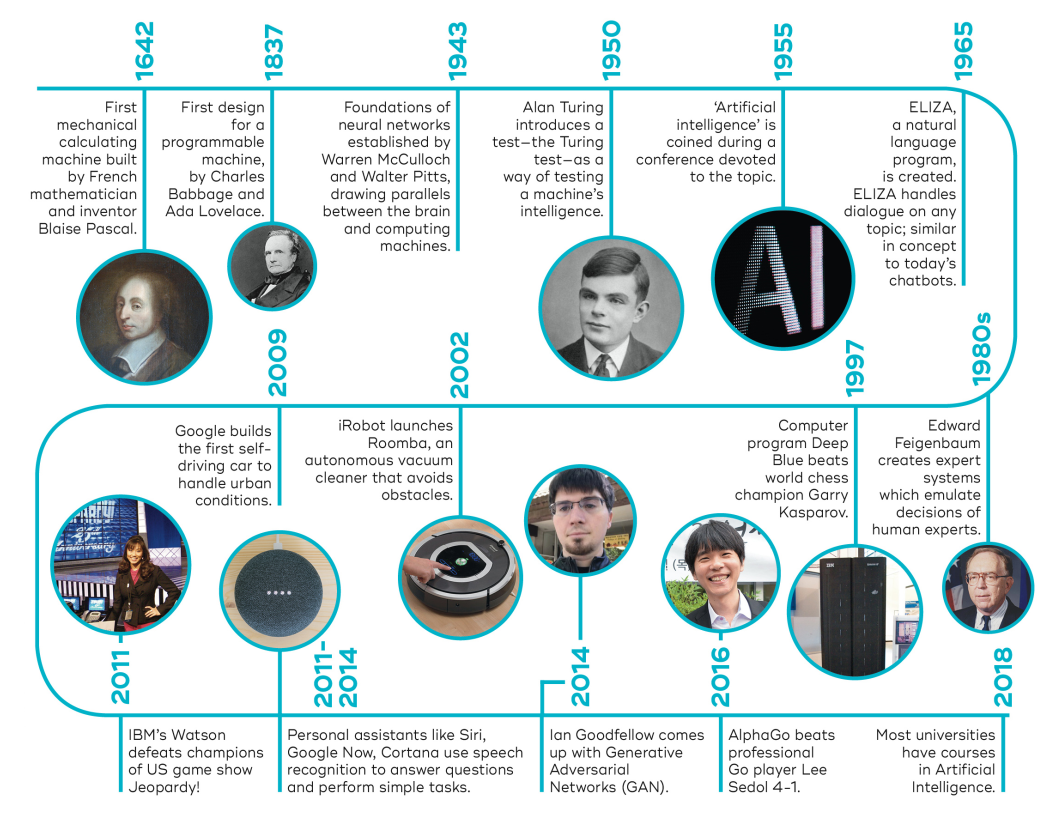
\includegraphics[width=0.5\textwidth]{ai-history.png}
    \caption{Geschiedenis van AI}
\end{figure}

Belangrijkste gebeurtenissen:

\begin{itemize}
    \item \textbf{1943:} McCulloch - Pitts: fundering van neurale netwerken
    \item \textbf{1950:} Alan Turing: de Turing test
    \item \textbf{1956:} Dartmouth workshop: bijeenkomst voor breinstorm AI
    \item \textbf{1997:} Garry Kasparov vs Deep Blue (IBM)
    \item \textbf{2011:} IBM Watson
    \item \textbf{2016:} AlphaGo
    \item \textbf{2021-:} toekomst
\end{itemize}

\subsubsection{Vormen van AI}

\begin{itemize}
    \item Zwakke AI (weak AI / Artificial Narrow Intelligence)
    \begin{itemize}
        \item Goed in een bepaalde taak maar alleen in die taak
        \item \textbf{Voorbeelden: } spamfilters, schaakcomputers, gezichtsherkenning
    \end{itemize}
    \item Sterke AI (strong AI / Artificial General Intelligence)
    \begin{itemize}
        \item Intelligentie op menselijk niveau
        \item In staat om zich aan te passen en problemen te leren oplossen in verschillende contexten
    \end{itemize}
    \item Superintelligentie (Artificial Super Intelligence)
    \begin{itemize}
        \item Als AI zelfbewust wordt en de mens op alle vlakken voorbij steekt
    \end{itemize}
\end{itemize}

\begin{figure}[H]
    \centering
    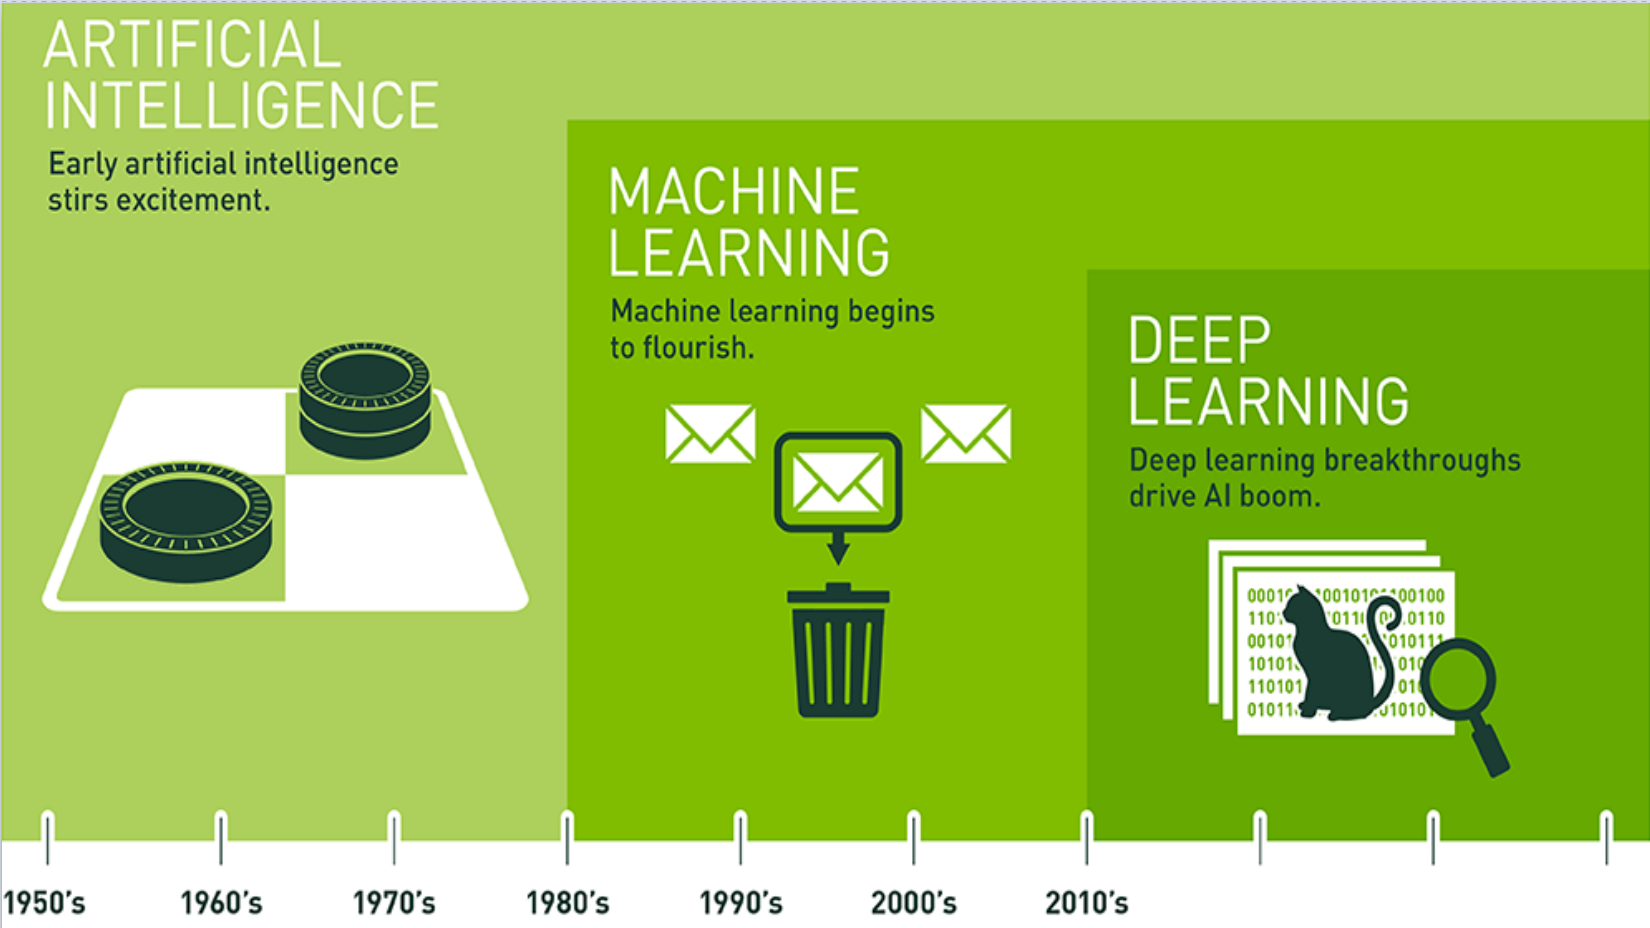
\includegraphics[width=0.6\textwidth]{ai-history2.png}
    \caption{AI vs ML vs DL}
\end{figure}

\subsubsection{Sectoren die de planeet verbeteren}

\begin{itemize}
    \item Klimaatsverandering
    \item Biodiversiteit en conservatie
    \item Water
    \item Hernieuwbare energie
    \item Medische sector
    \item Weer- en rampenvoorspelling
\end{itemize}

\subsubsection{Waarom nu?}

\begin{itemize}
    \item Snellere hardware
    \item Betere algoritmes
    \item Meer data
    \item (Open source) frameworks
\end{itemize}

\begin{figure}[H]
    \centering
    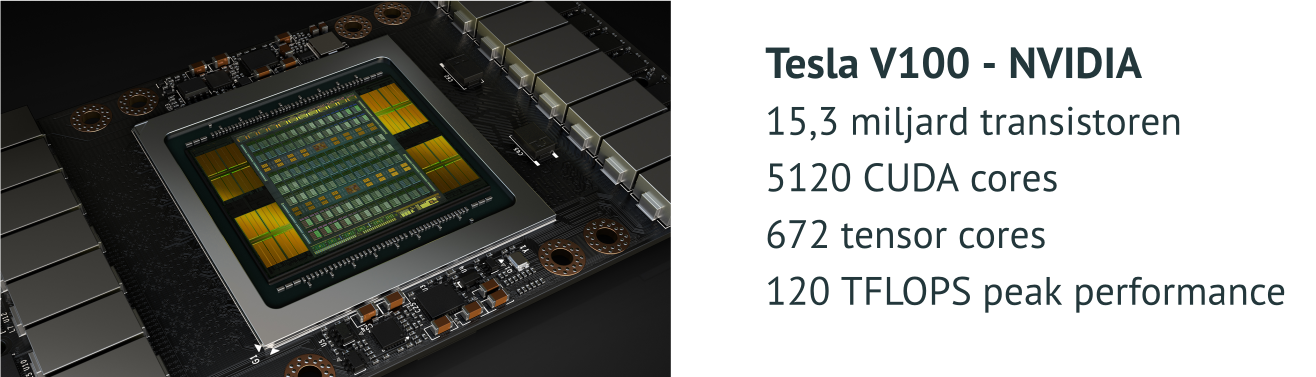
\includegraphics[width=0.5\textwidth]{nvidia-tesla.png}
    \caption{Voorbeeld huidige hardware: de Tesla V100 van Nvidia}
\end{figure}

\section{Hoe leren uit data?}

\subsection{Leeralgoritmes}

\begin{itemize}
    \item Supervised
    \begin{itemize}
        \item Inputs met gewenste outputs zijn gegeven
        \item Task driven
    \end{itemize}
    \item Unsupervised
    \begin{itemize}
        \item De gewenste outputs zijn niet gegeven
        \item Data driven (clustering)
    \end{itemize}
    \item Reinforcement
    \begin{itemize}
        \item Beslissingsproces op basis van beloningen
        \item Algoritme leert te reageren op zijn omgeving
    \end{itemize}
\end{itemize}

\begin{figure}[H]
    \centering
    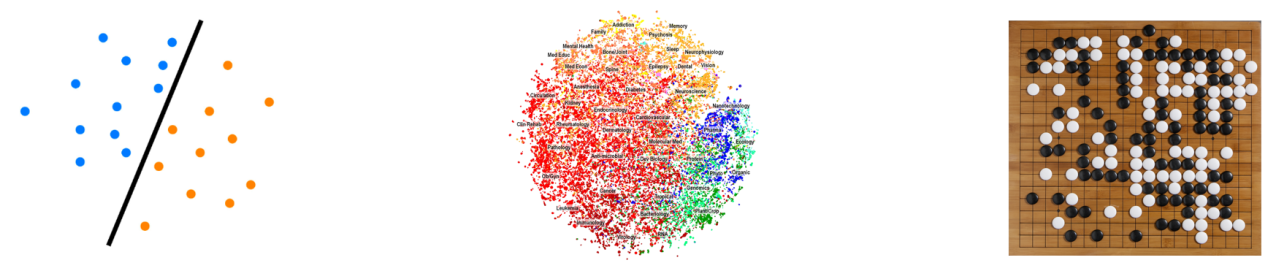
\includegraphics[width=0.5\textwidth]{leeralgoritmes.png}
    \caption{Supervised / Unsupervised / Reinforcement learning}
\end{figure}


\subsection{Supervised Learning}

Leren uit een gelabelde dataset. Vind het verband tussen de features en de labels

\begin{figure}[H]
    \centering
    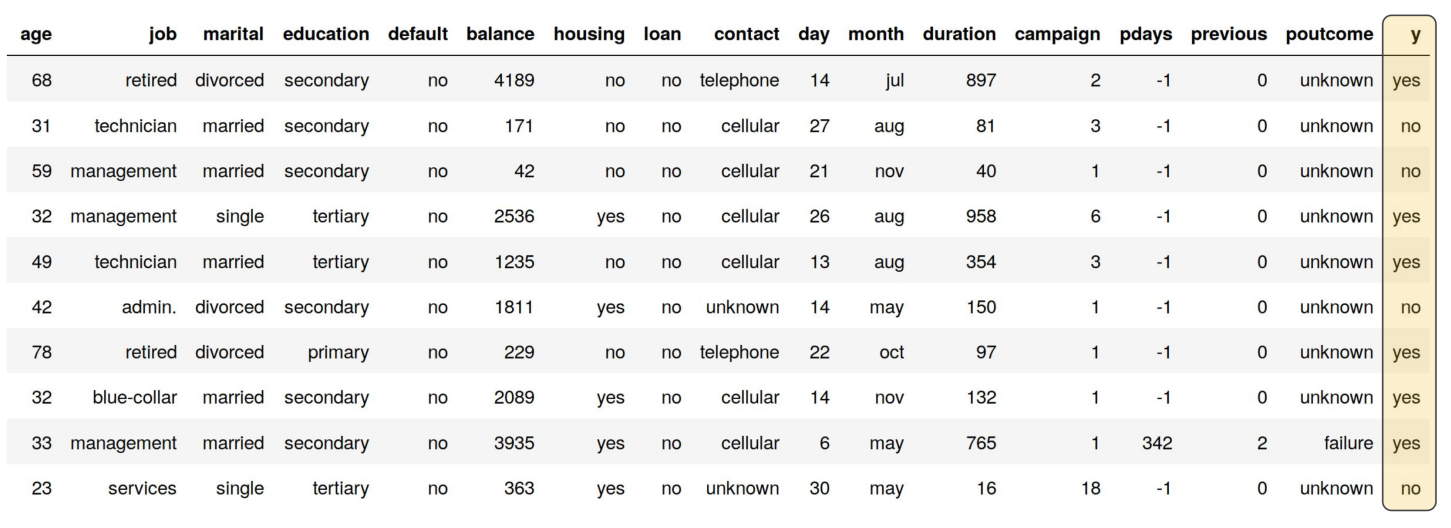
\includegraphics[width=0.5\textwidth]{supervised-learning.png}
    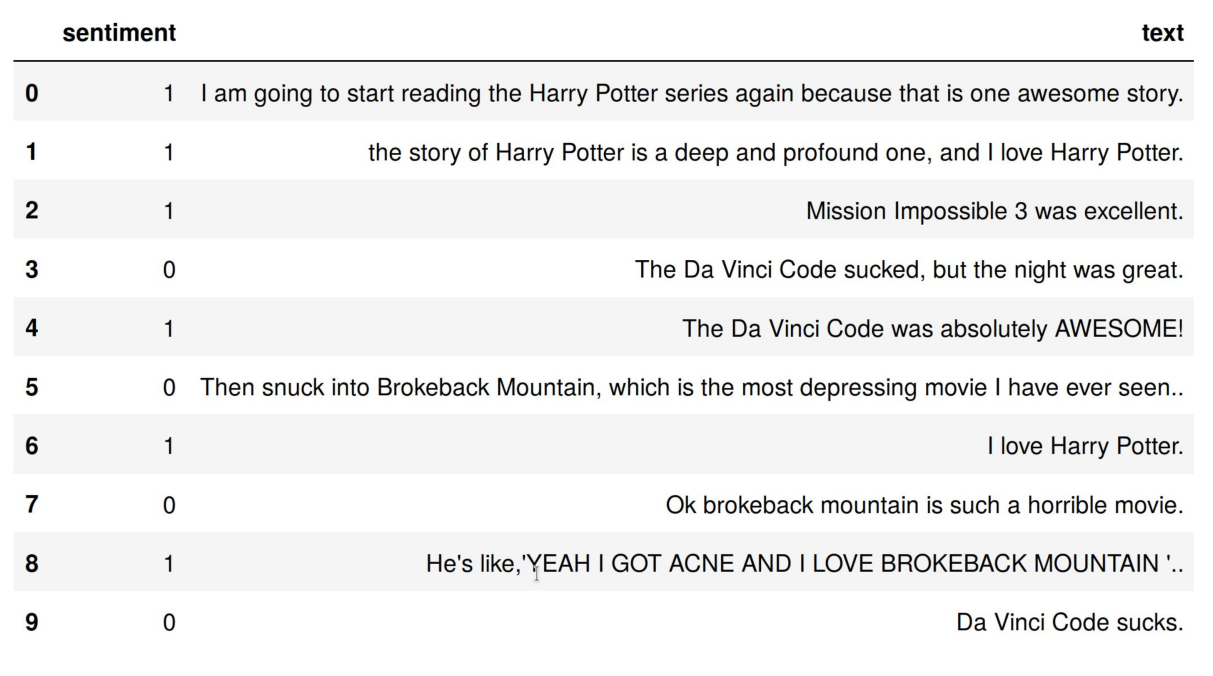
\includegraphics[width=0.4\textwidth]{supervised-learning2.png}
    \caption{Leren uit een dataset}
\end{figure}

\begin{figure}[H]
    \centering
    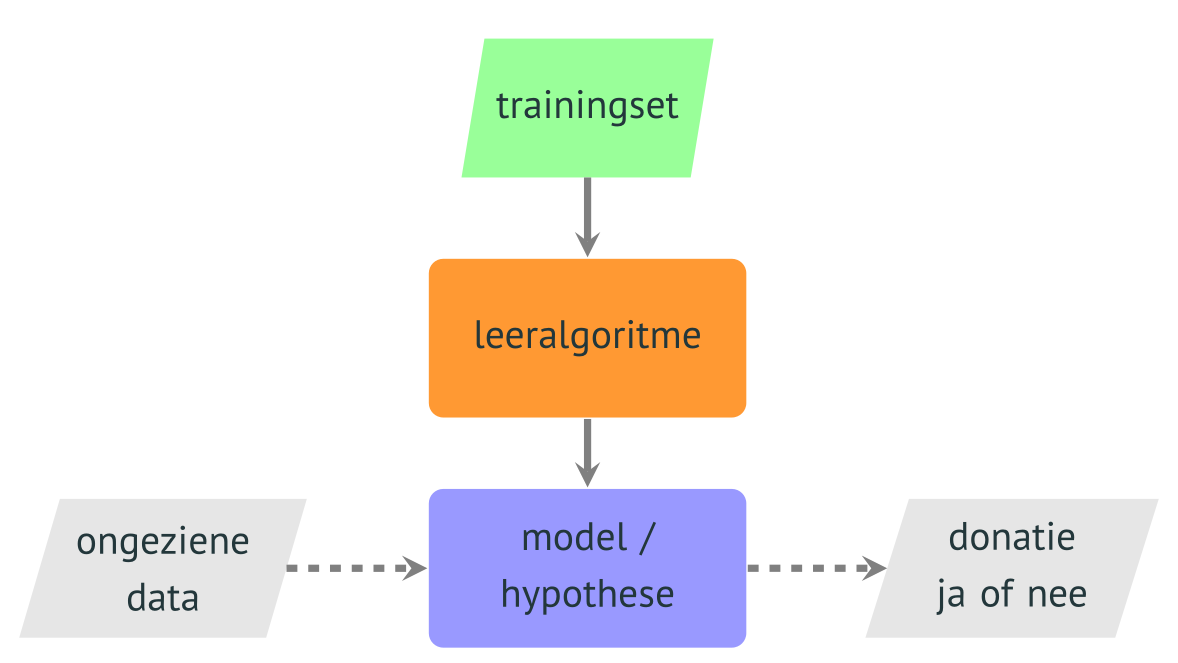
\includegraphics[width=0.5\textwidth]{supervised-learning3.png}
    \caption{Supervised learning kan uit ongeziene data een resultaat berekenen}
\end{figure}

\subsubsection{Regressie vs Classificatie}

\begin{figure}[H]
    \centering
    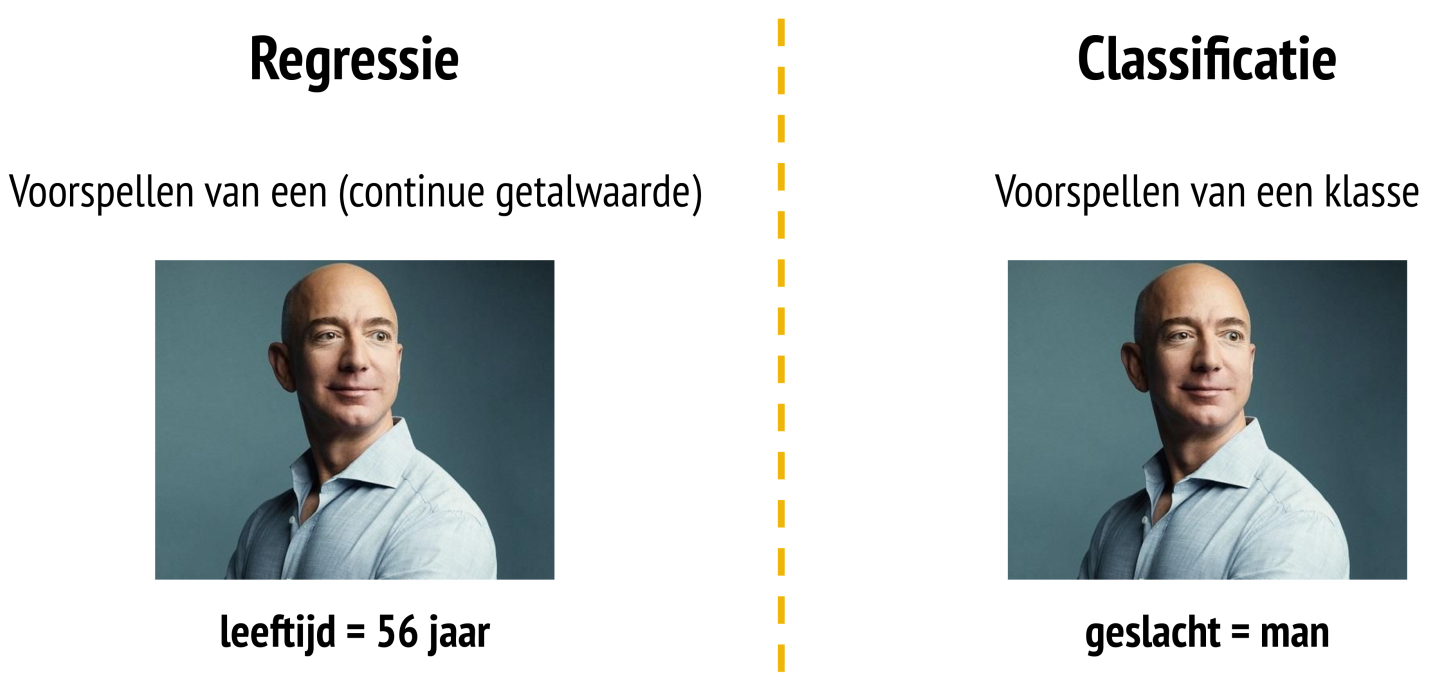
\includegraphics[width=0.5\textwidth]{regressie-vs-classificatie.png}
    \caption{Regressie vs classificatie}
\end{figure}

\begin{figure}[H]
    \centering
    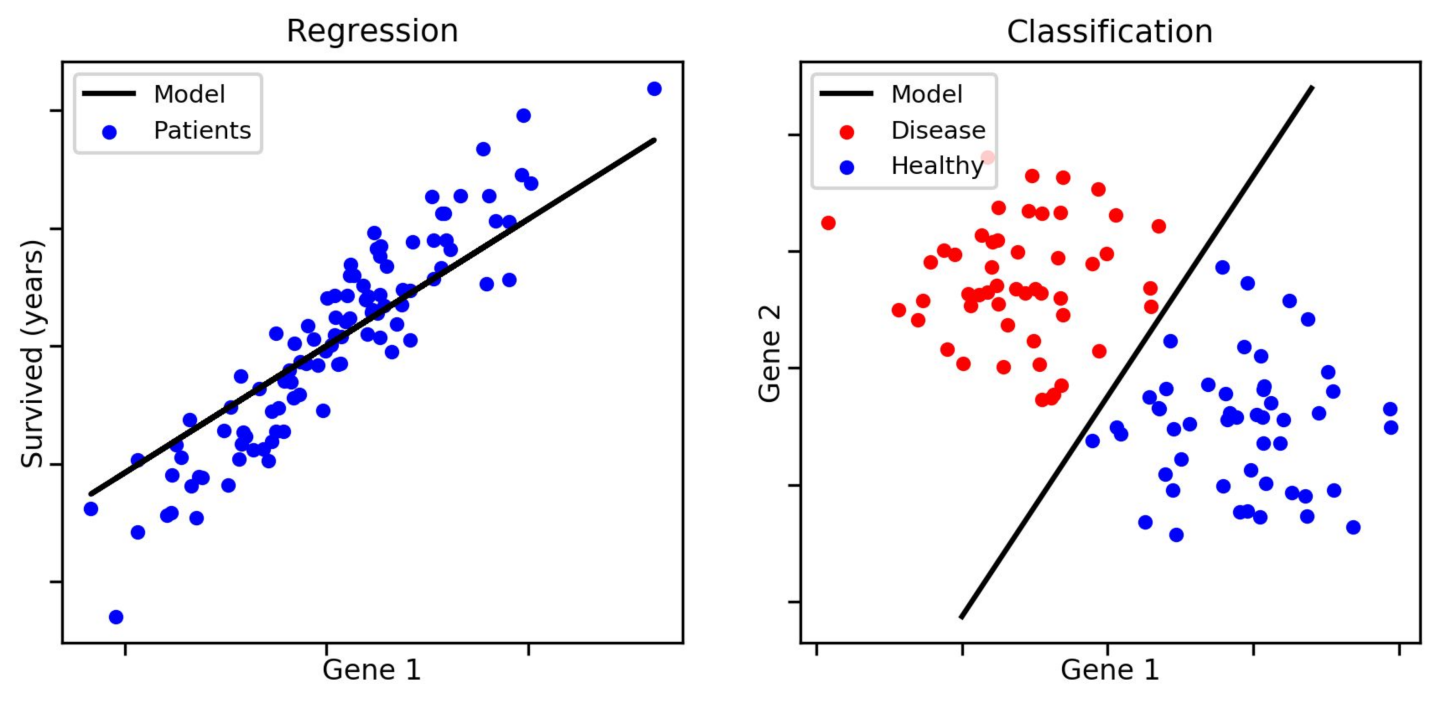
\includegraphics[width=0.5\textwidth]{regressie-vs-classificatie2.png}
    \caption{Regressie vs classificatie}
\end{figure}

\subsubsection{Voorbeeld}

Hoe stuurhoek bepalen bij een self-driving car?

\begin{itemize}
    \item (infrarood) camera's
    \item Stereo vision
    \item Radar
    \item LIDAR
    \item GPS
    \item Audio
\end{itemize}

\begin{figure}[H]
    \centering
    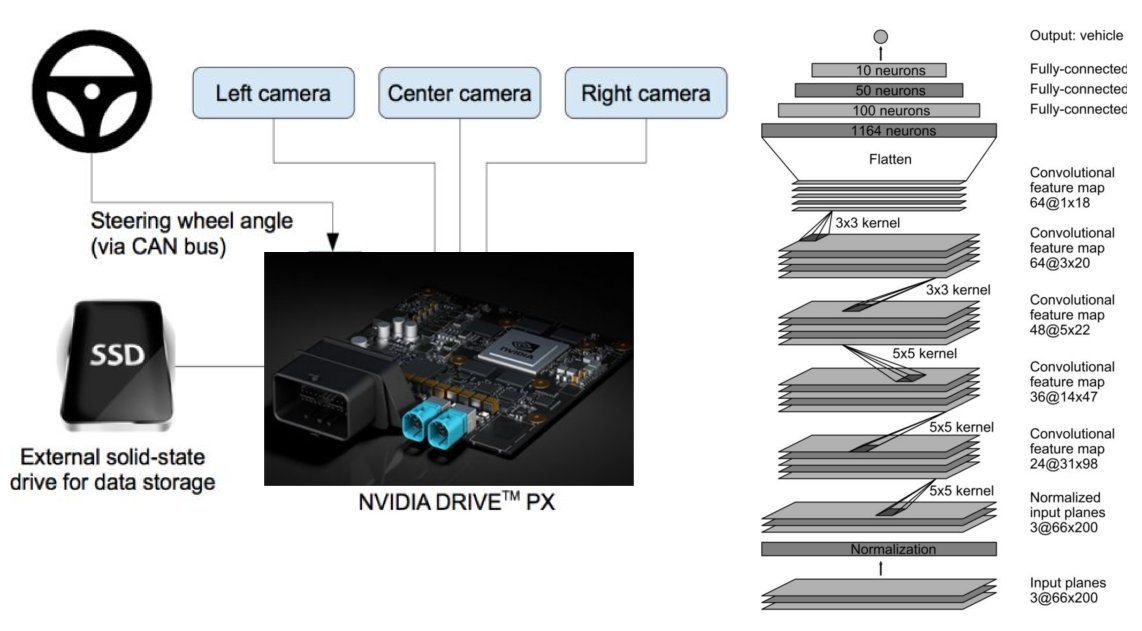
\includegraphics[width=0.6\textwidth]{stuurhoek-selfdriving-car.png}
    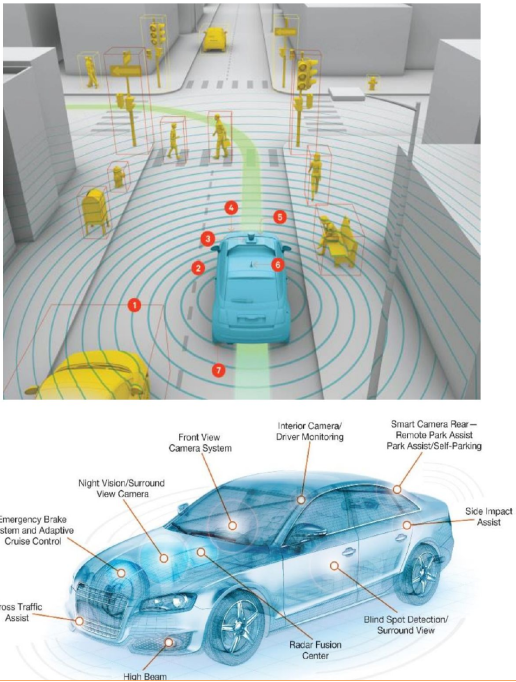
\includegraphics[width=0.3\textwidth]{stuurhoek-selfdriving-car2.png}
    \caption{Via sensoren weet de auto }
\end{figure}



\subsection{Unsupervised learning}

\begin{figure}[H]
    \centering
    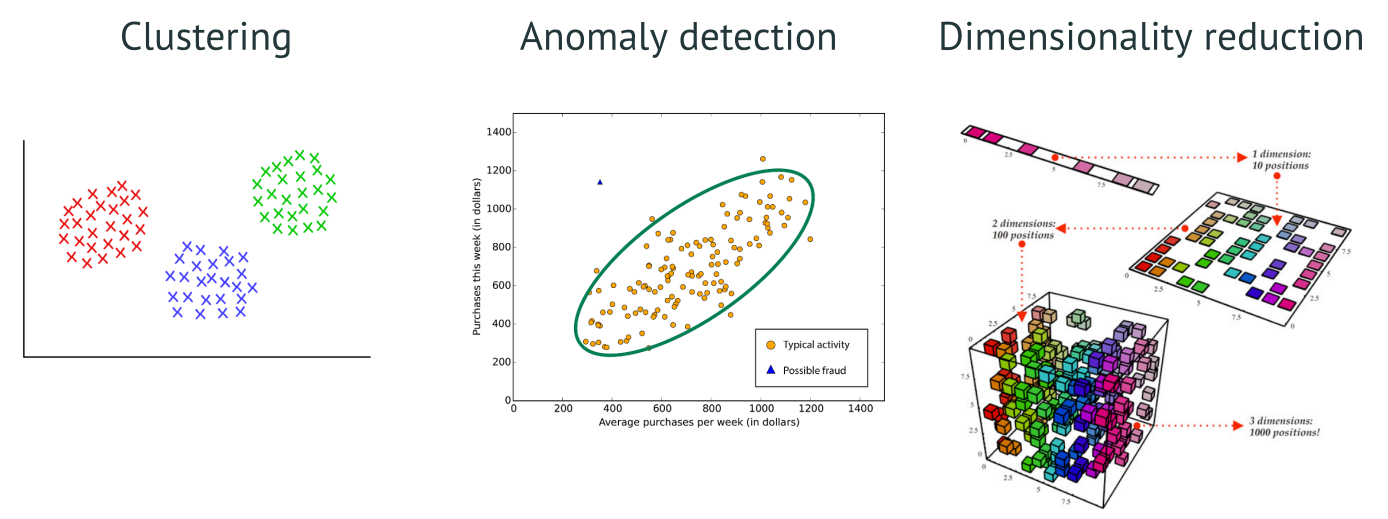
\includegraphics[width=0.7\textwidth]{unsupervised-learning.png}
    \caption{Unsupervised Learning}
\end{figure}

\begin{figure}[H]
    \centering
    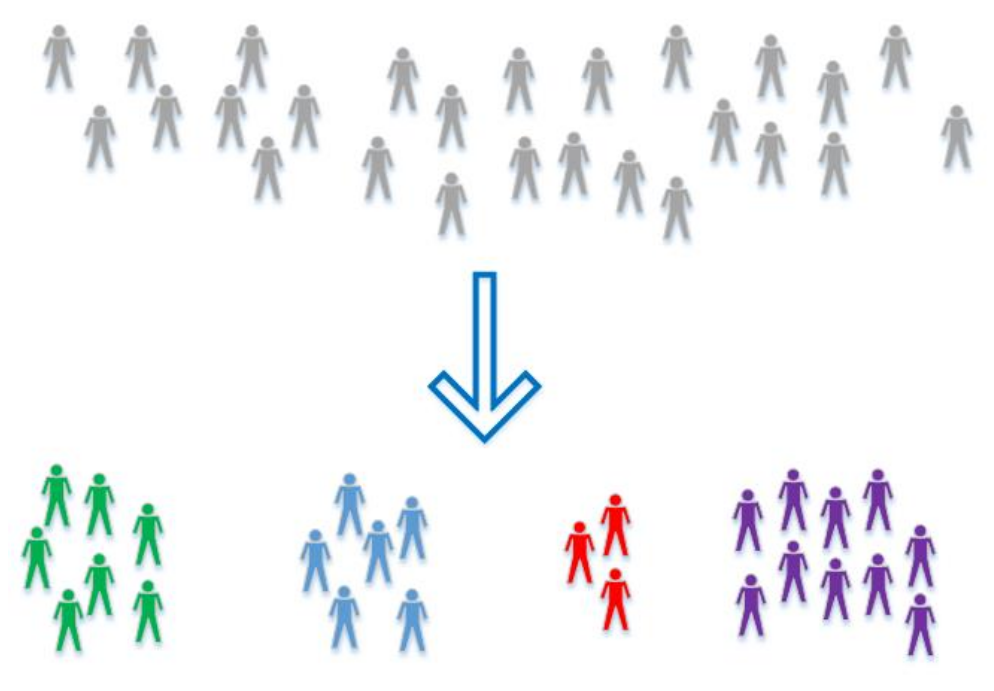
\includegraphics[width=0.5\textwidth]{unsupervised-learning2.png}
    \caption{Voorbeeld Clustering: de data in groepen verdelen}
\end{figure}

\subsection{Reinforcement learning}

\begin{figure}[H]
    \centering
    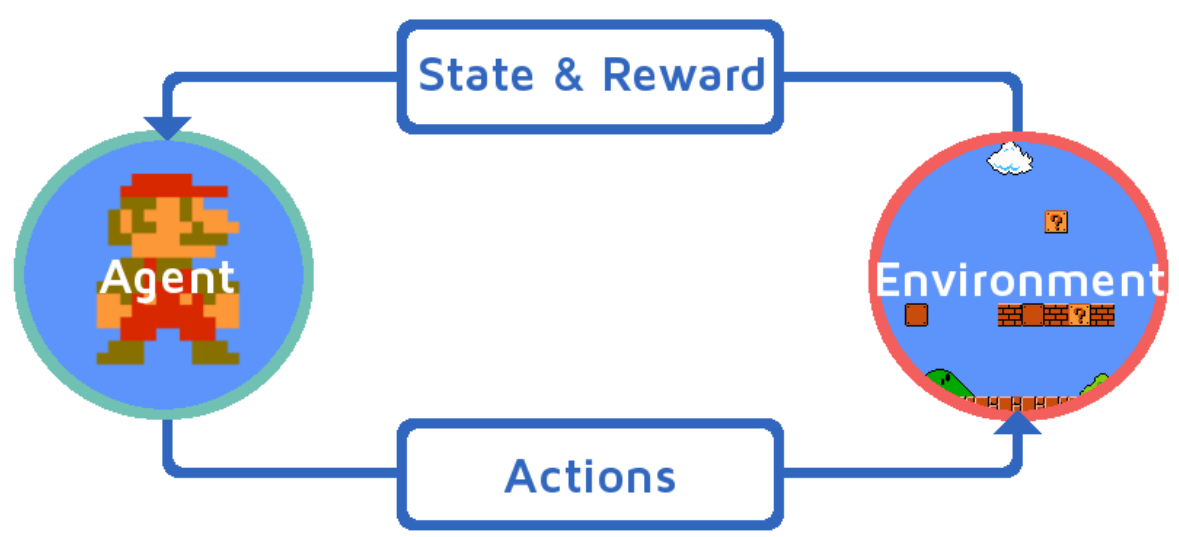
\includegraphics[width=0.5\textwidth]{reinforcement-learning.png}
    \caption{Reinforcement learning}
\end{figure}

\begin{itemize}
    \item Voor elke actie krijgt de AI feedback
    \item De AI leert uit de feedback
    \item In het begin zijn de acties heel willekeurig
\end{itemize}

\subsection{Overzicht leeralgoritmes}

\begin{figure}[H]
    \centering
    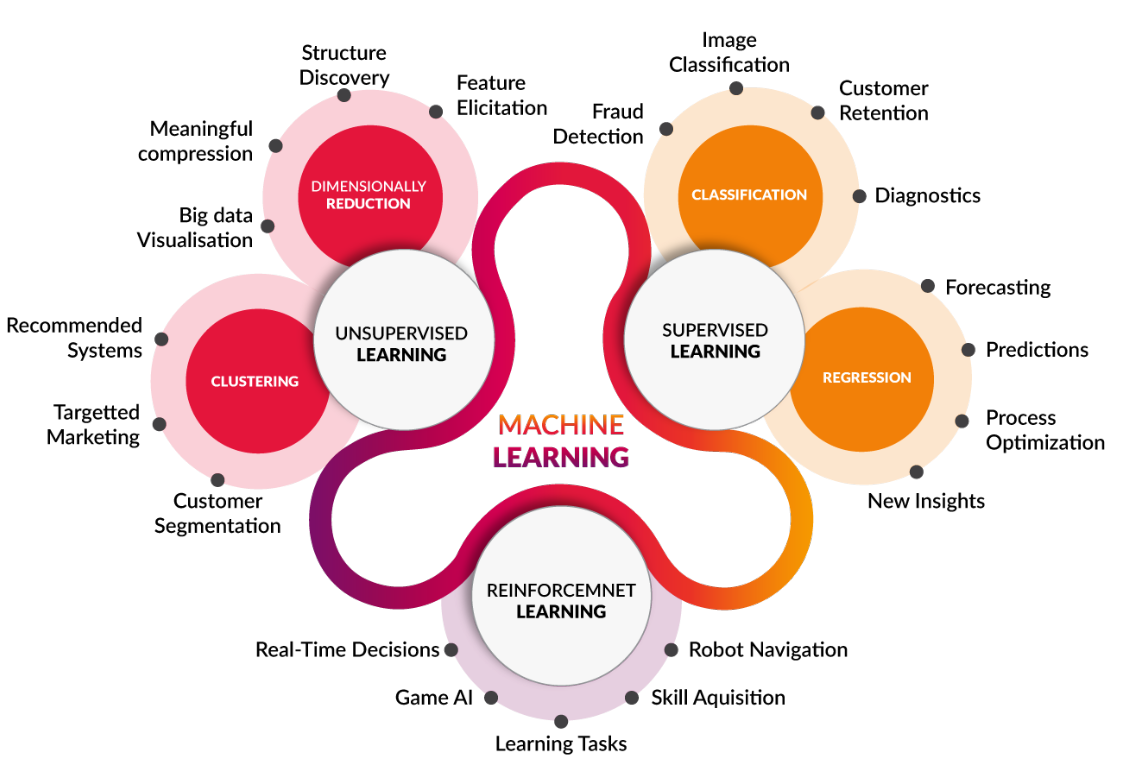
\includegraphics[width=0.55\textwidth]{overzicht-leeralgoritmes.png}
    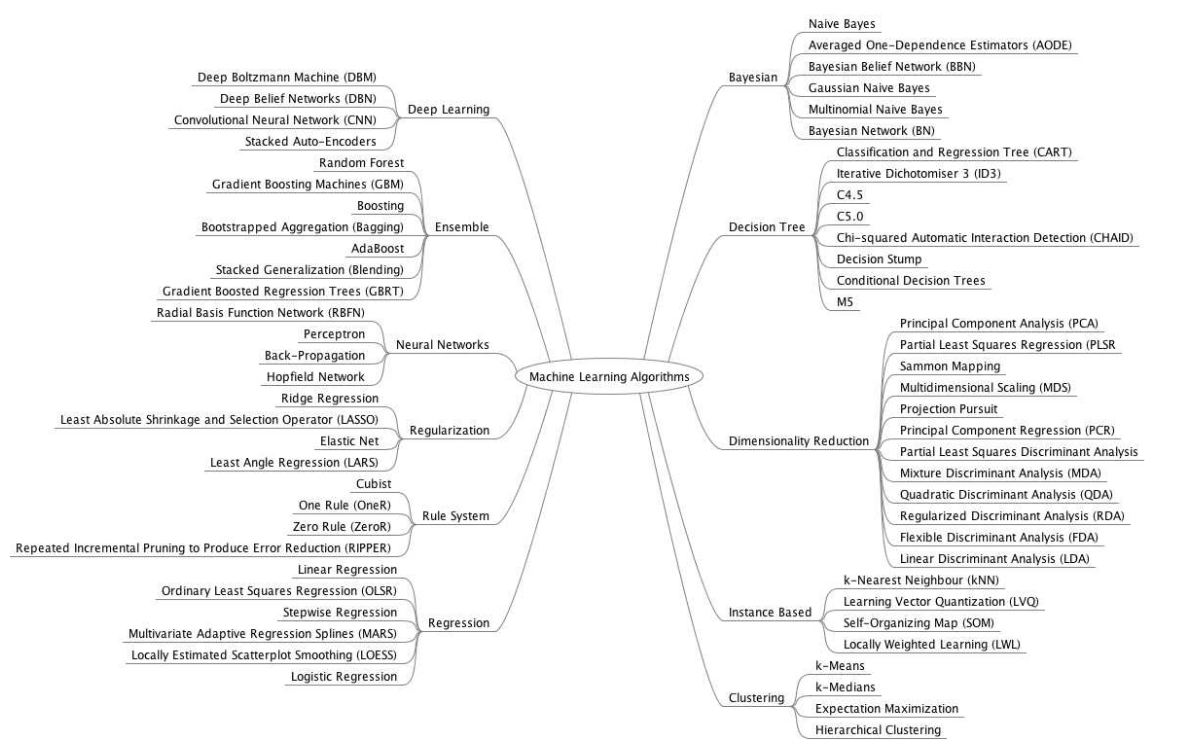
\includegraphics[width=0.5\textwidth]{overzicht-leeralgoritmes2.png}
    \caption{Overzicht}
\end{figure}

\subsection{Werkwijze van een ML Project}

\begin{figure}[H]
    \centering
    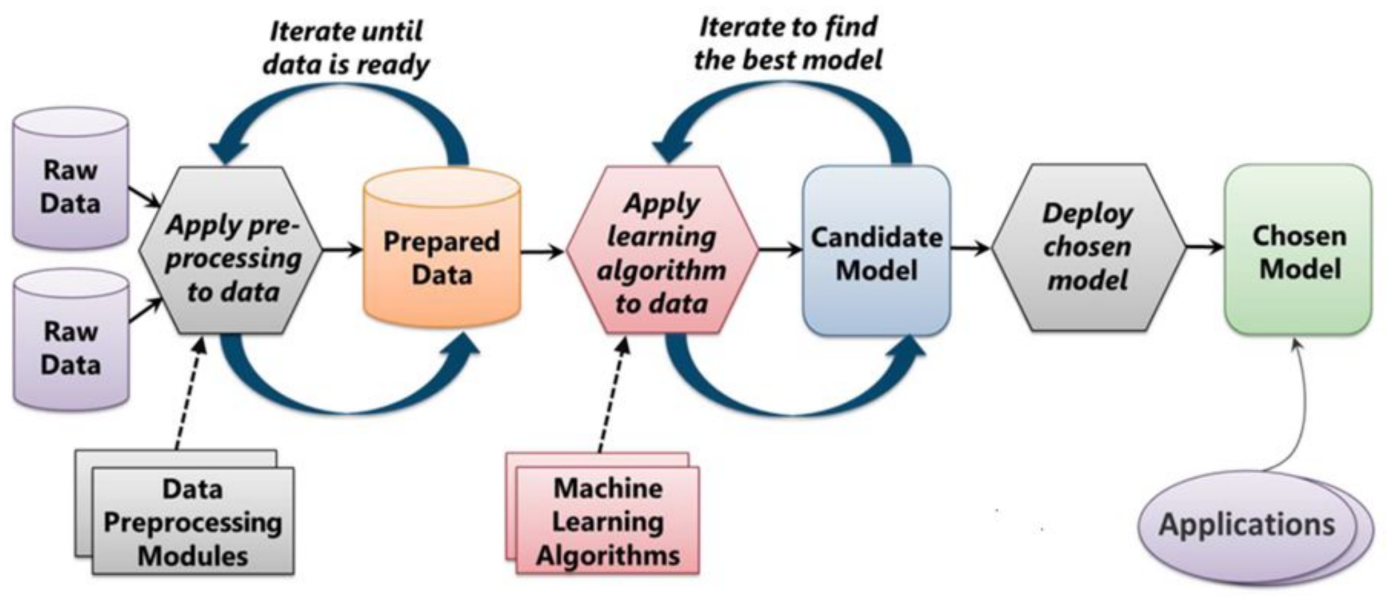
\includegraphics[width=0.4\textwidth]{machine-learning-project.png}
    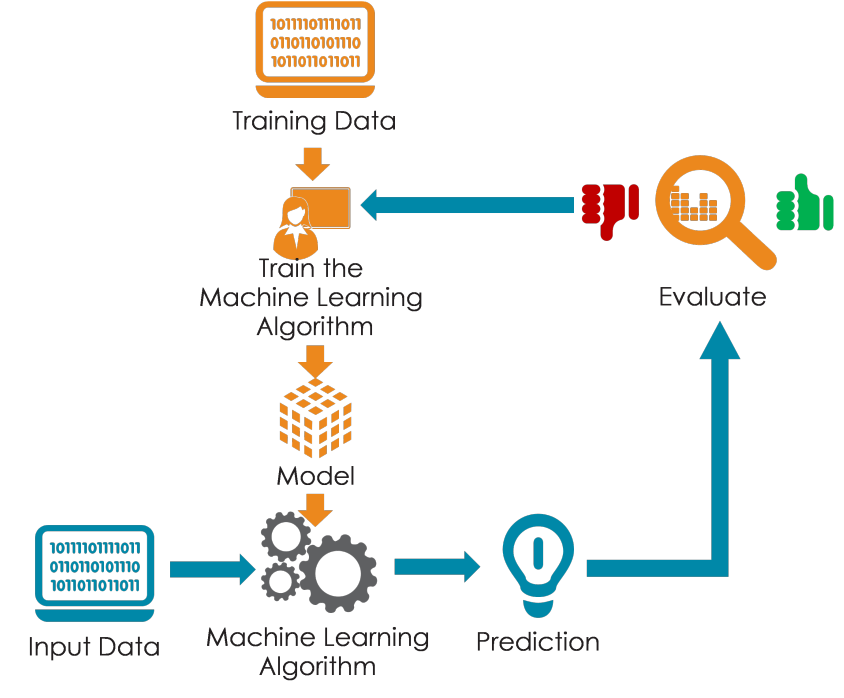
\includegraphics[width=0.35\textwidth]{machine-learning-project2.png}
    \caption{}
\end{figure}

\begin{figure}[H]
    \centering
    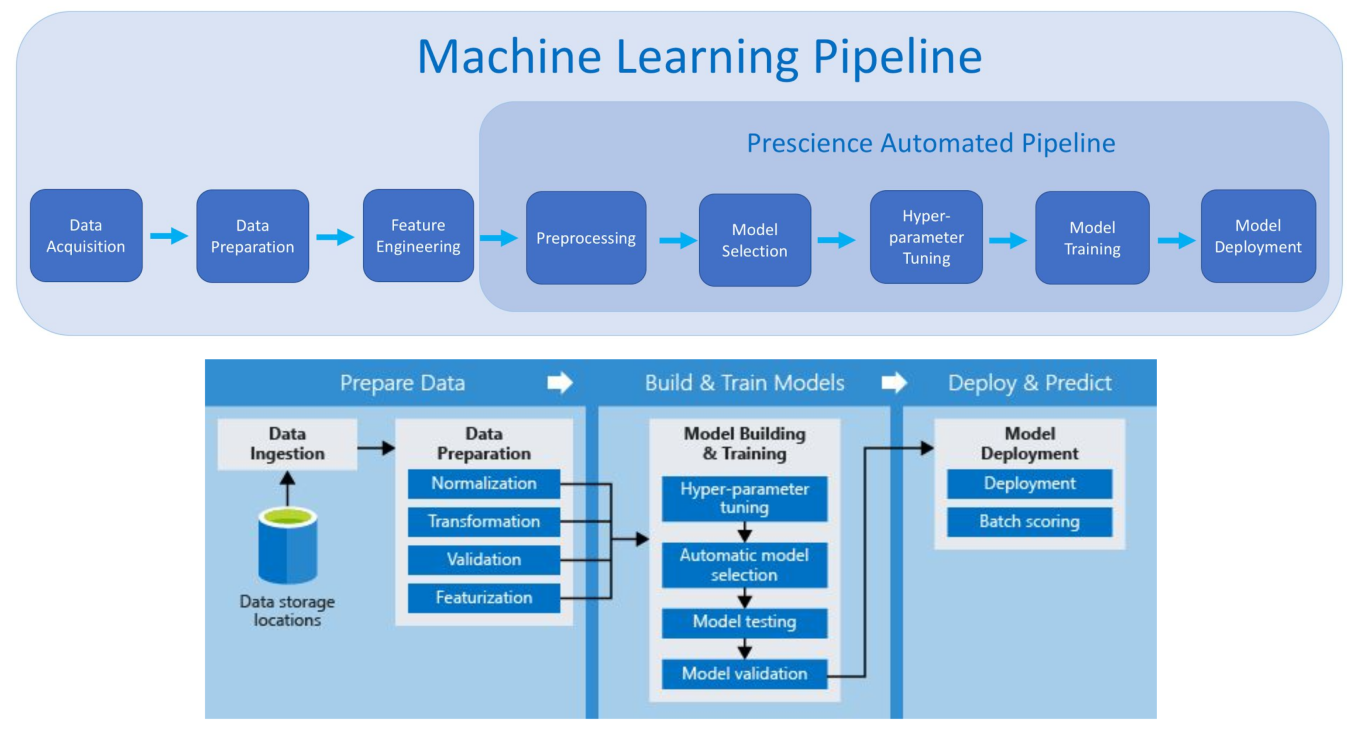
\includegraphics[width=0.45\textwidth]{machine-learning-project3.png}
    \caption{}
\end{figure}

\subsubsection{Tijdverdeling}


\begin{figure}[H]
    \centering
    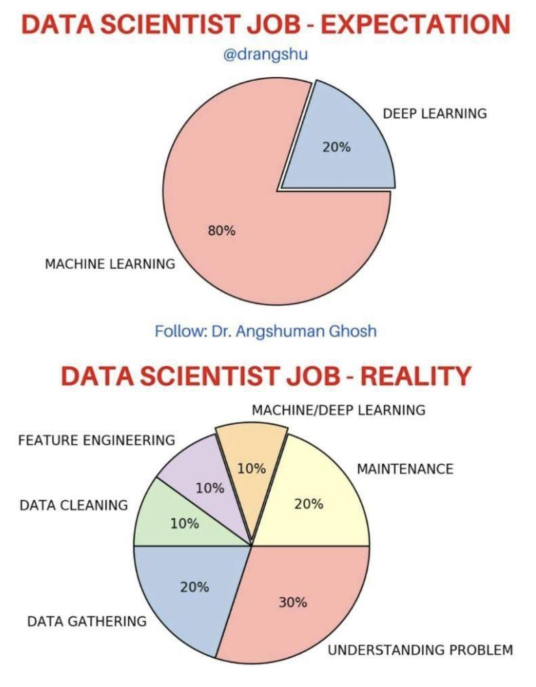
\includegraphics[width=0.35\textwidth]{machine-learning-project4.png}
    \caption{Tijdverdeling: verwachting vs realiteit}
\end{figure}

\section{Enkelvoudige Lineaire regressie}

\subsection{Voorbeeld}

\begin{figure}[H]
    \centering
    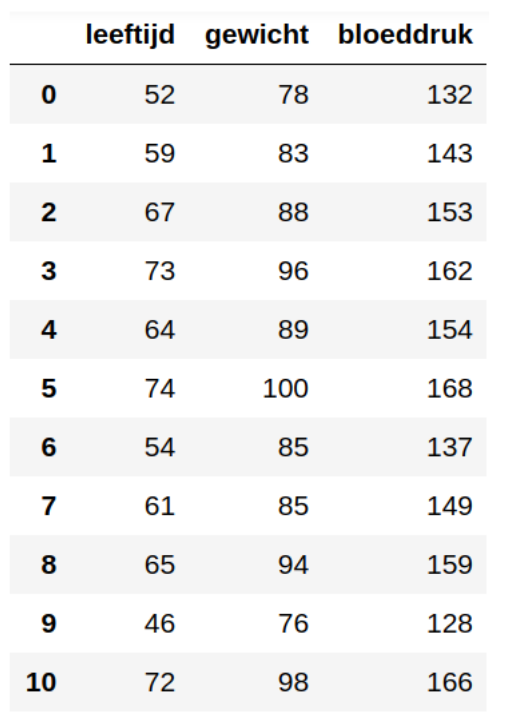
\includegraphics[width=0.3\textwidth]{lineaire-regressie-voorbeeld.png}
    \caption{Voorspel de bloeddruk op basis van leeftijd en gewicht}
\end{figure}

\begin{itemize}
    \item \textbf{features:} leeftijd en gewicht
    \item \textbf{target:} bloeddruk (=wat je wil voorspellen = output = label)
    \item \textbf{trainingset:} 11 training examples (=samples)
\end{itemize}

\begin{theorem}[Regressie-analyse]
Regressie-analyse is het modelleren van of het zoeken naar een verband op basis van één of meerdere variabelen.

Bij regressie is de output/target een (continue) variabele
\end{theorem}

\subsubsection{Scatterplot}

\begin{figure}[H]
    \centering
    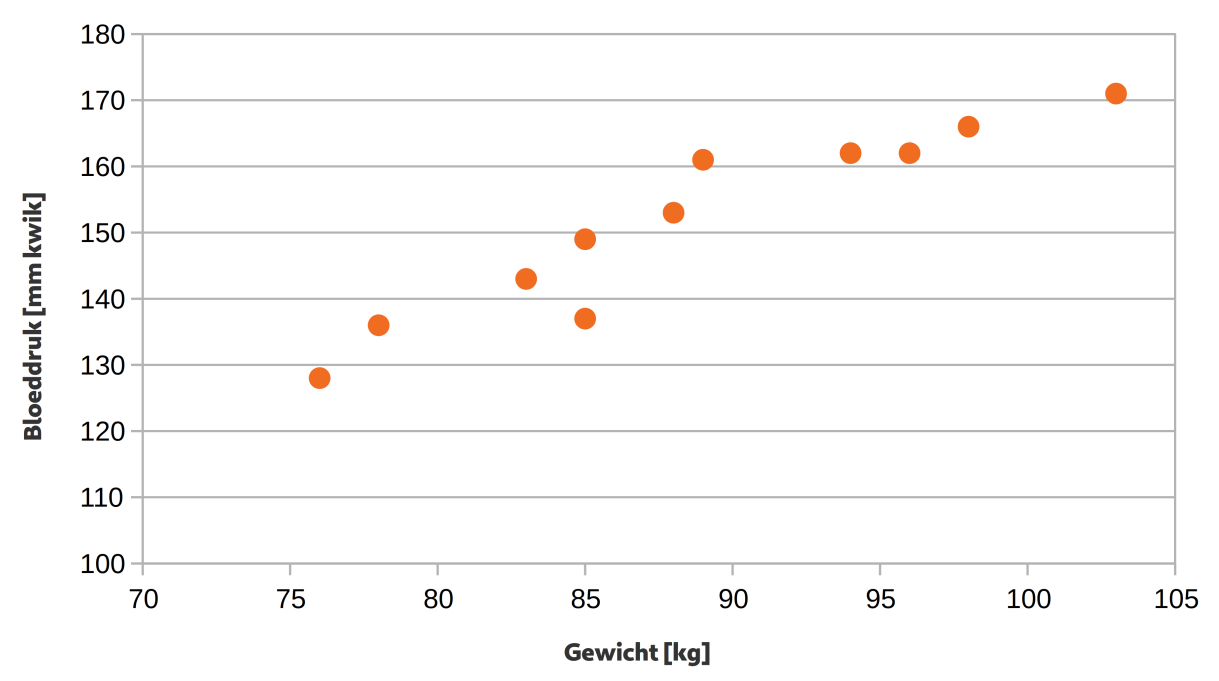
\includegraphics[width=0.5\textwidth]{lineaire-regressie-voorbeeld-scatterplot.png}
    \caption{Scatterplot: de grafiek toont een positieve correlatie $\Rightarrow$ een sterk verband}
\end{figure}

\subsection{De hypothese}

\begin{theorem}[De hypothese]
Het verband (model of hypothese) $h_{\theta}(x)$ is van de vorm:

\begin{equation}
h_{\theta}(x) = \theta_0 + \theta_1x
\end{equation}
\end{theorem}

Bepalen van de optimale waarden voor $\theta_0$ en $\theta_1$:

\begin{itemize}
    \item $\theta_0$ = snijpunt van de y-as (= noemen we ook de \textbf{bias})
    \item $\theta_1$ = helling van de rechte (rico)
\end{itemize}

De parameters $\theta_i$ = \textbf{weights}

Het zoeken van het model / hypothese = \textbf{training / learning}

\begin{figure}[H]
    \centering
    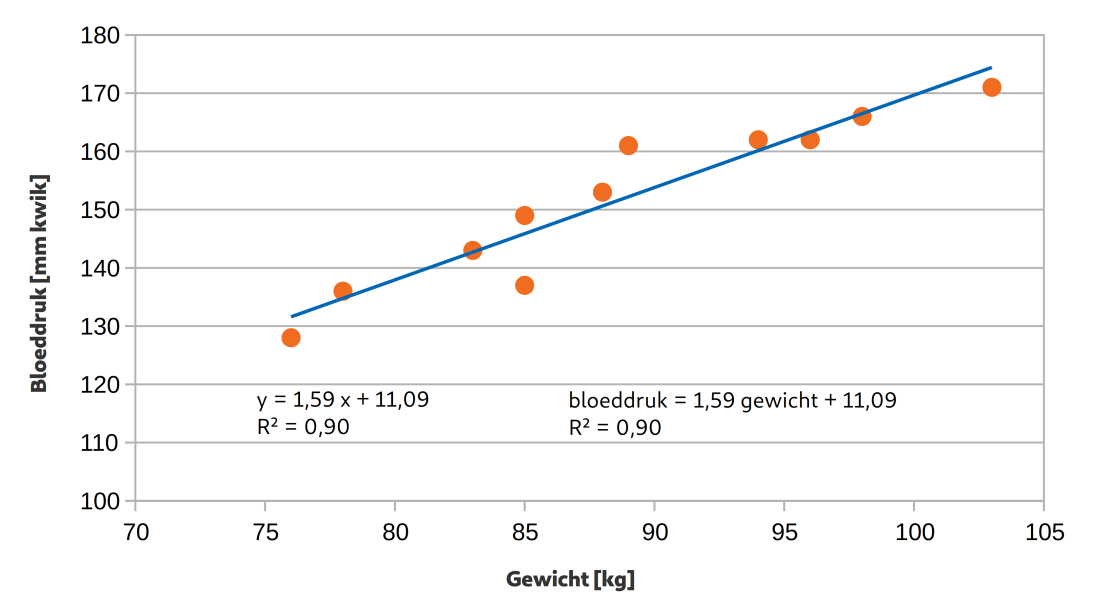
\includegraphics[width=0.5\textwidth]{lineaire-regressie-hypothese.png}
    \caption{Lineaire trnedlijn met model $h_{\theta}(x)$}
\end{figure}

$\mathbf{R^2}$\textbf{-waarde:} determinatiecoëfficiënt

\subsection{De kostenfunctie}

We moeten de kostenfunctie $J(\theta)$ via de \textbf{Least Mean Squared} methode (LMS). 

\begin{equation}
J(\theta) = \frac{1}{2\cdot m} \cdot \sum_{i=1}^m (h_{\theta}(x^{i}) - y^i)^2
\end{equation}

\begin{itemize}
    \item $m =$ de bias $=$ snijpunt met de y-as
    \item De kostenfunctie berekent de gemiddelde fout door alle fouten op te tellen
    \item Elke fout wordt gekwadrateerd om:
    \begin{itemize}
        \item negatieve waardes positief te maken
        \item de fout uit te groten
    \end{itemize}
\end{itemize}

\subsection{Gradient Descent (GDS)}

\begin{equation}
J(\theta_0, \theta_1) = \frac{1}{2\cdot m} \cdot \sum_{i=1}^m ((\theta_1\cdot x^i + \theta_0) - y^i)^2
\end{equation}

Stel de parameters $\theta_0$ en $\theta_1$ voortdurend bij in een iteratief proces 
tot je de waarden voor $\theta_0$ en $\theta_1$ hebt gevonden die de kleinst mogelijke waarde. Start met willekeurige waarden.

\begin{figure}[H]
    \centering
    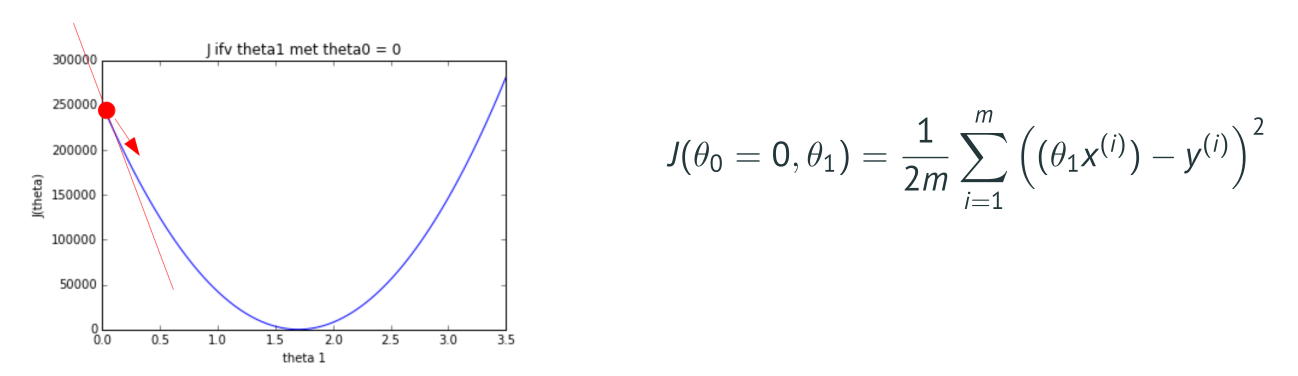
\includegraphics[width=0.5\textwidth]{gradient-descent-theta0.png}
    \caption{De GDS als $\theta_0 = 0$}
\end{figure}

\begin{itemize}
    \item Je krijgt een dalparabool als uitkomst 
    \item Je kan aflezen wat de parameters moeten zijn om de kleinst mogelijke waarde te vinden
    \item In de realiteit heb je vaak veel meer dan 2 gewichten
    \begin{itemize}
        \item Voorbeeld: de textgenererende AI GPT-3 heeft rond de 175 miljard gewichten 
        \item $\Rightarrow$ veel rekenkracht nodig om beste uitkomst te vinden
    \end{itemize}
\end{itemize}

\subsubsection{Learning rate}

\begin{figure}[H]
    \centering
    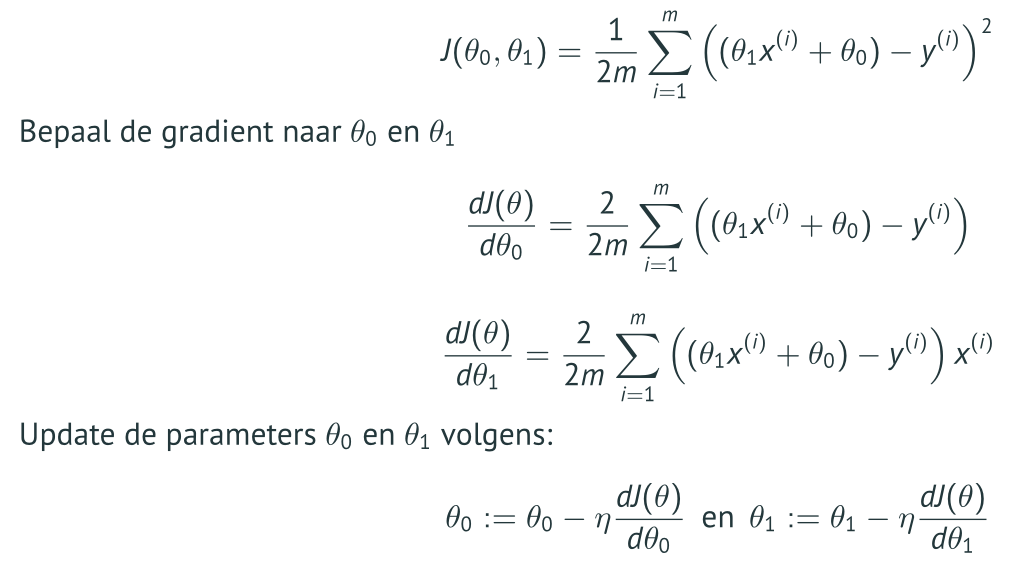
\includegraphics[width=0.65\textwidth]{gradient-descent-afgeleiden.png}
    \caption{De parameters $\theta_0$ en $\theta_1$ stellen we constant bij (formules niet te kennen)}
\end{figure}

\begin{itemize}
    \item We bepalen de afgeleide (= de gradient, de helling) van $\theta_0$ en $\theta_1$
    \item We gebruiken die afgeleiden om een betere $\theta_0$ en $\theta_1$ te vinden.
    \item We vermenigvuldigen de gradient met een variable $\eta$ (=de learning rate)
    \item Onze nieuwe $\theta$ wordt berekend met behulp van de oude $\theta$ en de afgeleide maal de learning rate. 
\end{itemize}

\begin{figure}[H]
    \centering
    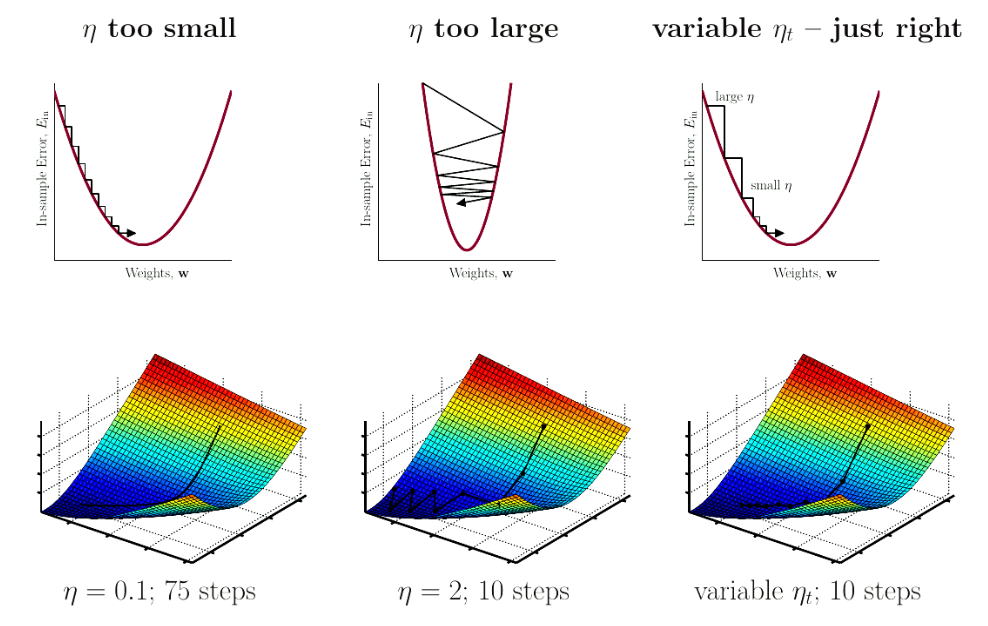
\includegraphics[width=0.5\textwidth]{lineaire-regressie-learning-rate.png}
    \caption{Learning rate $\eta$: bij een te kleine/te grote $\eta$ hebben we te veel stappen}
\end{figure}

De learning rate $\eta$ stellen we constant bij om met zo weinig aantal stappen het optimum te bereiken.


\section{Meervoudige lineaire regressie}

\begin{theorem}[Meervoudige lineaire regressie]
Bij meervoudige lineaire regressie (multiple regression) wordt het model/hypothese bepaald 
aan de hand van een trainingset met \textbf{meerdere features}.
\end{theorem}

\begin{itemize}
    \item Bloeddruk wordt bepaald a.d.h.v. gewicht en leeftijd
    \item De kwaliteit van wijn wordt voorspeld op basis van: zuurtegraad, suikergehalte, chloriden, dichtheid, sulfaten, hoeveelheid alcohol, \dots
    \item Het warmeverlies van een huis wordt voorspeld op basis van: het type glas, muurisolatie, oriëntatie van het huis, \dots
\end{itemize}

\begin{equation}
h_{\theta}(x) = \theta_0 + \theta_1x_1 + \theta_2x_2 + \dots + \theta_nx_n + 
\end{equation}

\begin{figure}[H]
    \centering
    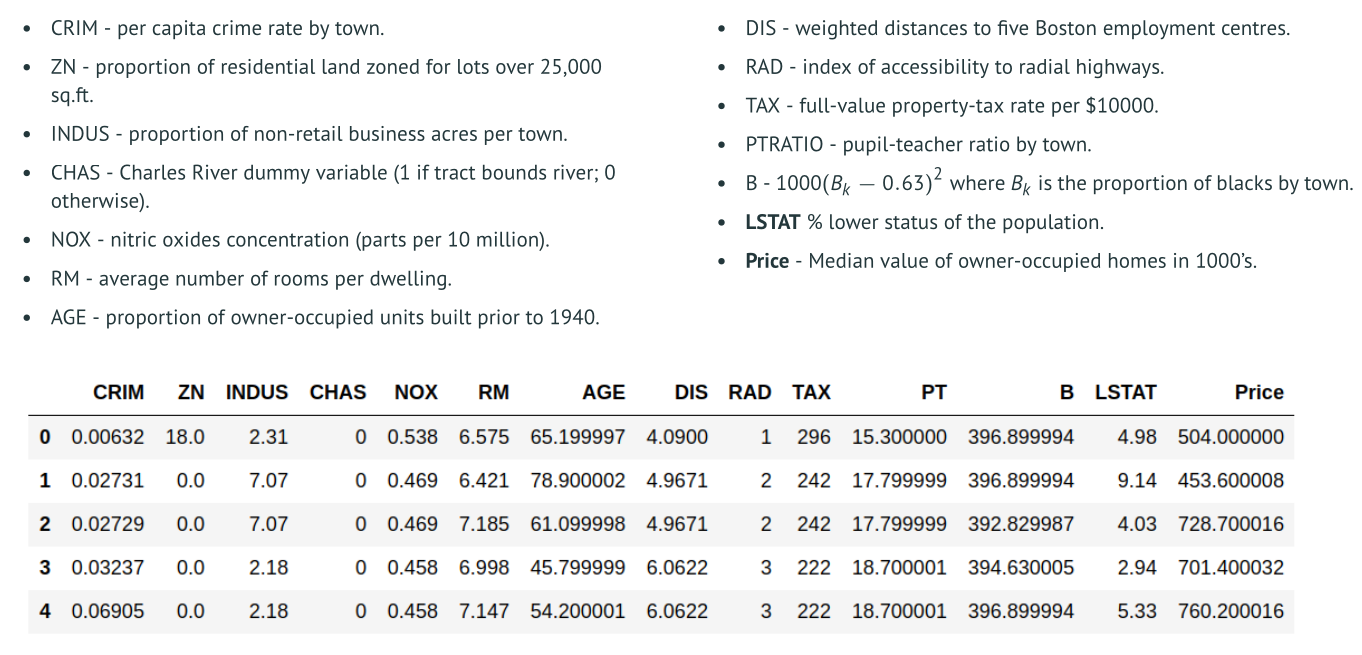
\includegraphics[width=0.7\textwidth]{multiple-regression-voorbeeld.png}
    \caption{\textbf{Voorbeeld:} voorspel de huisprijs op basis van deze features }
\end{figure}

\subsection{Statistische vooranalyse}

\subsubsection{Consistentie van de dataset}

\begin{itemize}
    \item Volledigheid van de dataset
    \item Inconsistenties
    \item Spreiding van de gegevens
\end{itemize}

We verwijderen de CHAS kolom:

\begin{minted}{python}
dataset.drop('CHAS', axis=1, inplace=True)
\end{minted}


\subsubsection{Uitschieters}

\begin{itemize}
    \item Vinden en verwijderen van extreme waarden/samples
    \item Geavanceerde technieken: zie later bij clustering
\end{itemize}

\begin{figure}[H]
    \centering
    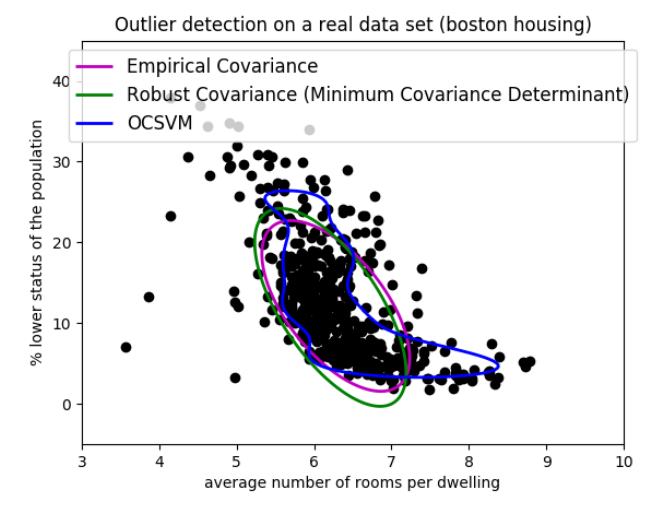
\includegraphics[width=0.5\textwidth]{multiple-regression-uitschieters.png}
    \caption{Uitschieters}
\end{figure}


\subsubsection{Onderlinge correlatie}

\begin{figure}[H]
    \centering
    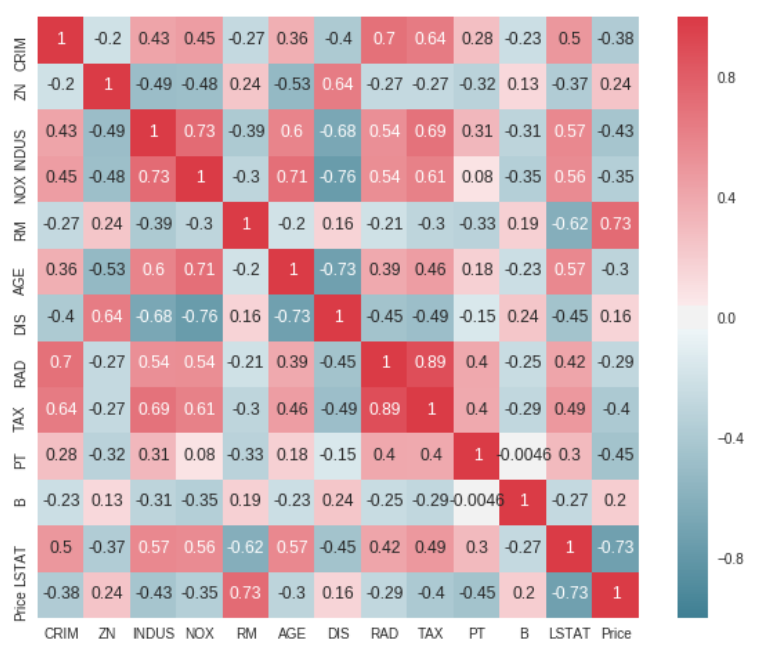
\includegraphics[width=0.45\textwidth]{multiple-regression-heatmap.png}
    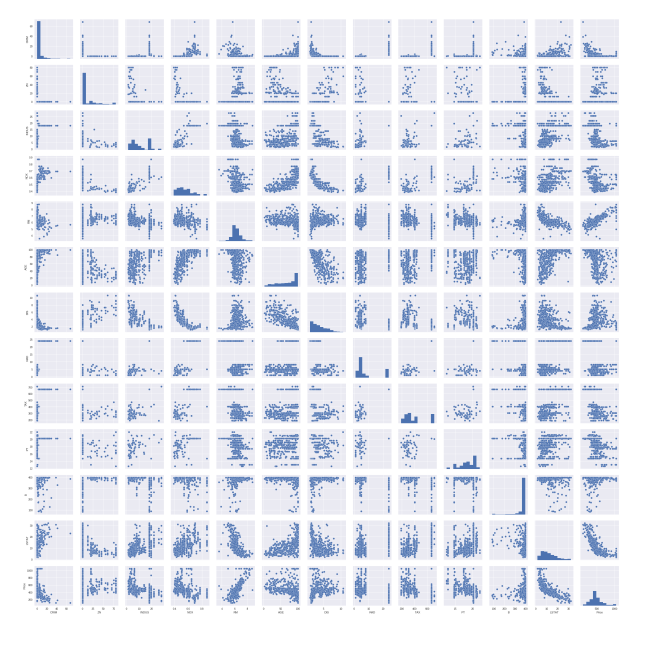
\includegraphics[width=0.45\textwidth]{multiple-regression-pairplot.png}
    \caption{Heatmap en pairplot van de onderline correlatie tussen de features}
\end{figure}

\subsection{Features en targets}

\begin{figure}[H]
    \centering
    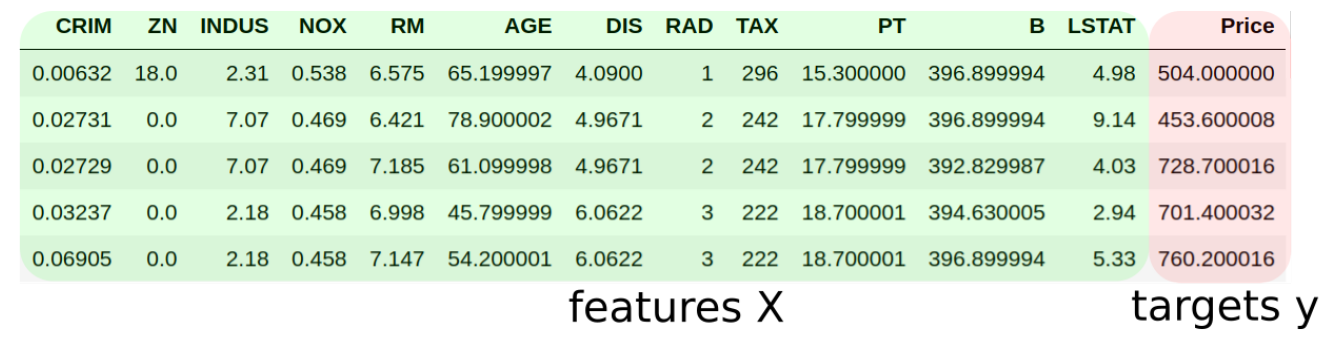
\includegraphics[width=0.5\textwidth]{multiple-regression-features-targets.png}
    \caption{Dataset opsplitsen in features en targets}
\end{figure}

\begin{minted}{python}
y = dataset['target_kolom'].values
X = dataset.drop('target_kolom',axis=1).values
# Alternatief
features=list(dataset.columns[:dataset.columns.size-1])
X = dataset[features].values
y = dataset['Price'].values
\end{minted}

\subsection{Trainen van het model}

\begin{figure}[H]
    \centering
    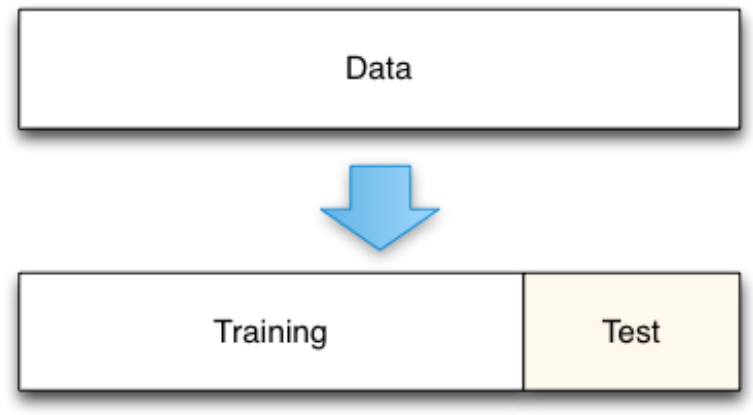
\includegraphics[width=0.5\textwidth]{multiple-regression-training-testset.png}
    \caption{Dataset opsplitsen in training set en test set}
\end{figure}

\begin{itemize}
    \item Belangrijk om eerst de data te randomiseren: te data zou gesorteerd kunnen zijn, dat willen we vermijden
    \item Stel dat huizenprijzen van laag naar hoog gesorteerd is, en je traint de data op de eerste 75\%, en test de laatste 25\%.
    Resultaat: Het model zal niet getraind zijn op dure huizen.
    \item Ander voorbeeld: stel dat je een self-driving AI alleen traint op de autosnelweg, en dan test in een zone-30 straat bij een school...
\end{itemize}


\begin{minted}{python}
X_train, X_test, y_train, y_test = train_test_split(X, y, test_size=0.33, 
random_state=0)
\end{minted}

\subsubsection{Initialiseren en trainen van het regressiemodel}

\begin{minted}{python}
lregmodel = linear_model.LinearRegression()
lregmodel.fit(X_train, y_train)
\end{minted}

Model:

\begin{minted}{python}
print('coeffs: ', lregmodel.coef_)
print('intercept', lregmodel.intercept_)

>> coeffs: [ -3.56141289e+00, 4.05479295 e-01, 8.14080284 e-01, 
    8.96450415 e+01, -3.02997261e-01, -2.77339444e+01, 
    7.47151897 e+00, -2.92233040e-01, -1.61741146e+01, 
    -1.17962045e +01]

>> intercept: 650.652022517
\end{minted}

Price = - 3.56 × CRIM + 0.41 × ZN + 0.81 × INDUS - 270.51 × NOX + 89.65 × RM
- 0.30 × AGE - 27.74 × DIS + 7.47 × RAD - 0.29 × TAX - 16, 17 × PT
+ 0.08 × B - 11.80 × LSTAT + 650.65


\subsection{Testen van het model}

\subsubsection{Voorspellingen maken}

\begin{figure}[H]
    \centering
    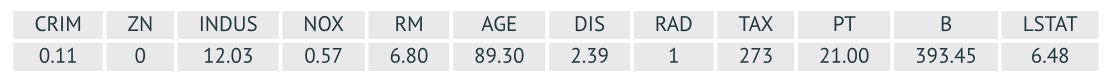
\includegraphics[width=0.5\textwidth]{multiple-regression-voorspelling.png}
    \caption{Voorspel de prijs van een huis met deze features}
\end{figure}

\begin{minted}{python}
house = np.array([0.11, 0, 12.03, 0.57, 6.80, 89.30, 2.39, 1, 
273, 21.00, 393.45, 6.48])

house = house.reshape(1, -1)

# met reshape wordt house:
# house = np.array([[0.11, 0, 12.03, 0.57, 6.80, 89.30, 2.39, 1, 
# 273, 21.00, 393.45, 6.48]])

price = lregmodel.predict(house)

print('De prijs van het huis bedraagt: ', price)

>> De prijs van het huis bedraagt: 563.68335073
\end{minted}

\begin{itemize}
    \item reshape(1, -1) maakt een rijvector
    \item Werkelijke prijs: 562.00
\end{itemize}

\subsection{Performantie en scores van het model}

\subsubsection{Mean Absolute Error (MAE)}

\begin{theorem}[MAE]
De Mean Absolute Error (MAE) is \textbf{het gemiddelde van de absolute waarden} van het verschil
tussen de \textbf{werkelijke waarden} $y_i$ en de \textbf{voorspelde waarden} $\hat{y}_i$.

\begin{equation}
\text{MAE} = \frac{1}{n} \cdot \sum_{i=1}^n | y_i - \hat{y}_i |
\end{equation}
\end{theorem}

\begin{minted}{python}
from sklearn.metrics import mean_absolute_error

y_predicted = lgregmodel.predict(X_test)
MAE = mean_absolute_error(y_test, y_predicted)

print('MAE= ', MAE)

>> MAE = 64.0090867586

\end{minted}

\subsubsection{Mean Squared Error (MSE)}

\begin{theorem}[MSE]
De Mean Squared Error (MSE) is \textbf{het gemiddelde van de gekwadrateerde waarden} van het verschil tussen de werkelijke waarden $y_i$ en
de voorspelde waarden $\hat{y}_i$.

\begin{equation}
\text{MSE} = \frac{1}{n} \cdot \sum_{i=1}^n ( y_i - \hat{y}_i )^2
\end{equation}
\end{theorem}

\begin{minted}{python}
from sklearn.metrics import mean_squared_error

y_predicted = lregmodel.predict(X_test)
MSE = mean_squared_error(y_test, y_predicted)

print('MSE = ' MSE)

>> MSE = 7803.89332739
\end{minted}


\subsubsection{Determinatiecoëfficiënt}

\begin{theorem}[De determinatiecoëfficiënt $R^2$]
De determinatiecoëfficiënt ($R^2$) is de variabiliteit van het model

\begin{equation}
R^2 = 1 - \frac{\sum_{i=1}^n (y_i - \hat{y}_i)^2 }{\sum_{i=1}^n (y_i - \bar{y})^2}
\end{equation}

Bij perfecte voorspellingen is $R^2 = 1$

Een negatieve waarde voor $R^2$ betekent dat het model slechter scoort dan een horizontale lijn (= slechter dan het gemiddelde te nemen) ($y_i = \bar{y}$, $\bar{y}$ is het gemiddelde van y)
\end{theorem}

\begin{minted}{python}
from sklearn.metrics import r2_score

y_predicted = lregmodel.predict(X_test)
r2 = r2_score(y_test, y_predicted)

print('r2_score = ', r2)

# alternatieve manier voor het bepalen van de r2 score:
r2 = lregmodel.score(X_test, y_test)

>> r2 score = 0.754254234917
\end{minted}

\section{Feature engineering}

Om een beter model te verkrijgen (en zo een betere $R^2$ score), kunnen we verschillende dingen doen:

\begin{itemize}
    \item Meer data toevoegen
    \item Ander model kiezen, hyperparameter tuning
    \item Feature engineering 
\end{itemize}

\subsection{Normalisatie / Scaling}

\begin{theorem}[Normalisatie / Scaling]
Normalisatie of Scaling zorgt ervoor dat de features op dezelfde schaalverdeling staan
\end{theorem}

In ons voorbeeld van de huurprijs:

\begin{figure}[H]
    \centering
    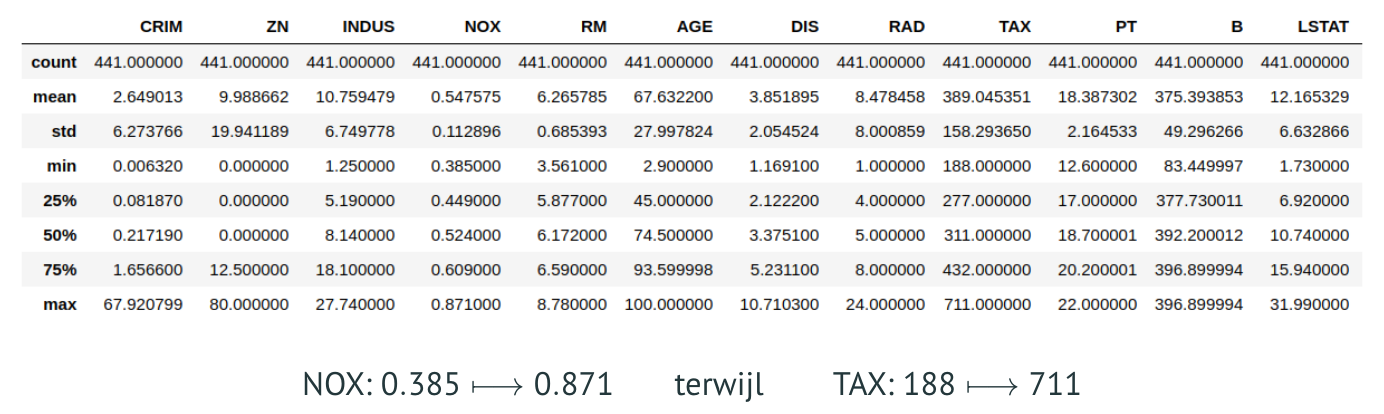
\includegraphics[width=0.6\textwidth]{normalisatie.png}
    \caption{NOX: min = 0.385, max = 0.871; TAX: min = 188, max = 711}
\end{figure}

\subsubsection{Voordelen}

\begin{figure}[H]
    \centering
    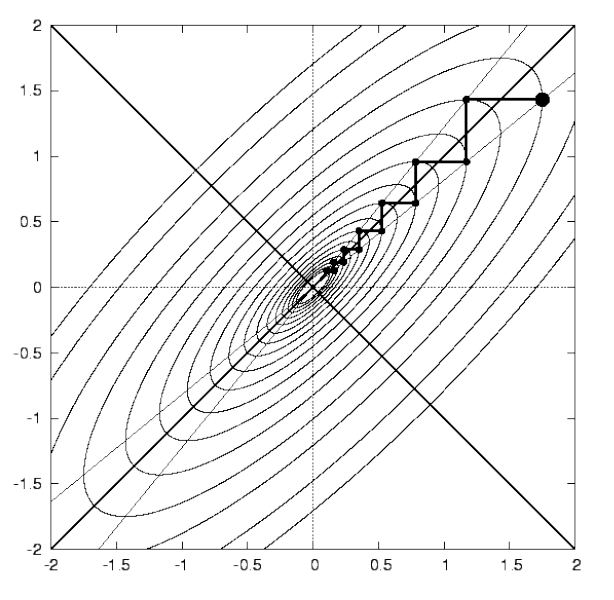
\includegraphics[width=0.4\textwidth]{scaling.png}
    \caption{Gradient Descent convergeert minder snel als features op een verschillende schaalgrootte staan. Normalisatie zorgt er dus voor dat het model sneller zal trainen.}
\end{figure}

\subsubsection{MIN-MAX-scaling}

\begin{equation}
x_{s_i} = \frac{x_i - Min(x)}{Max(x) - Min(x)}
\end{equation}

\begin{itemize}
    \item Schaalt alle features tussen 0 en 1
    \item Werkt goed bij niet-Gaussiaanse distributies en bij kleine variantie
    \item De scheefheid (skew) blijft bewaard
    \item Gevoelig voor uitschieters
\end{itemize}

\begin{figure}[H]
    \centering
    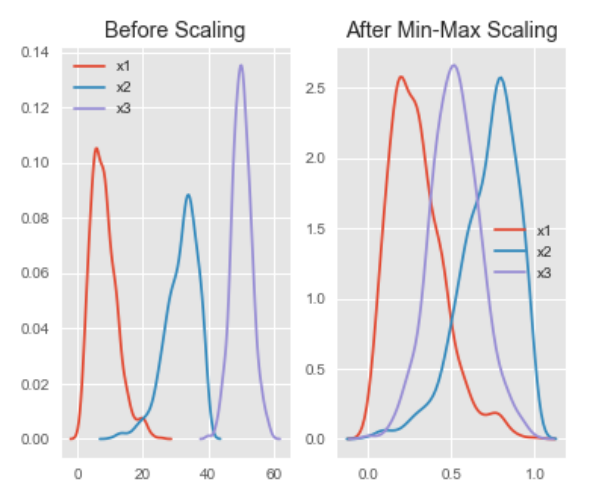
\includegraphics[width=0.4\textwidth]{min-max-scaling.png}
    \caption{Voor en na scaling}
\end{figure}

\begin{figure}[H]
    \centering
    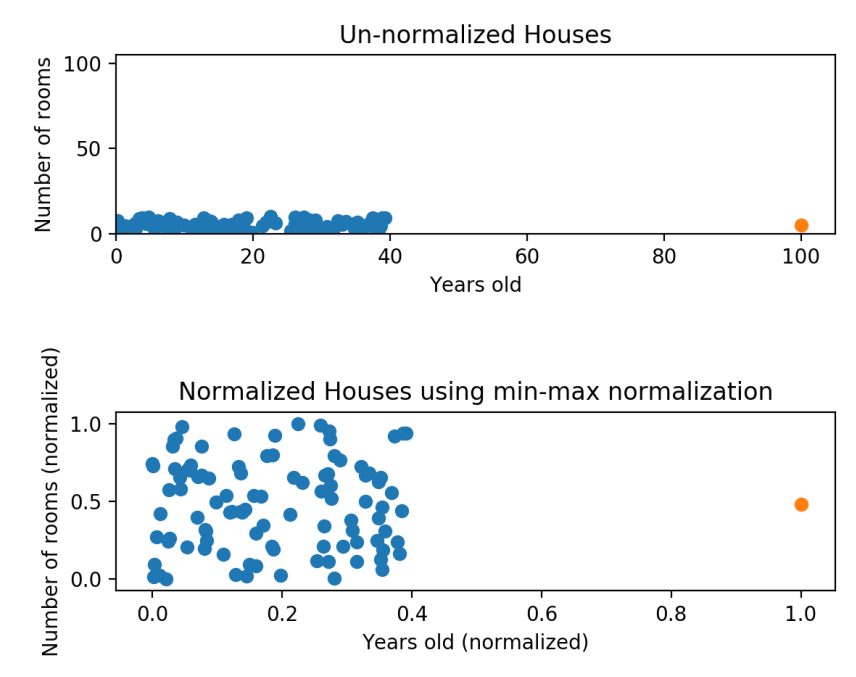
\includegraphics[width=0.4\textwidth]{min-max-houses.png}
    \caption{Bij het voorbeeld van de huizenprijzen}
\end{figure}

\begin{minted}{python}
from sklean.preprocessing import MinMaxScaler

scaler = MinMaxScaler.fit(X_train)
X_train = scaler.transform(X_train)
X_test = scaler.transform(X_test)

# alternatief
scaler = MinMaxScaler()
X_train = scaler.fit_transform(X_train)
X_test = scaler.transform(X_test)
\end{minted}

\subsubsection{Standard scaling (normalisatie)}

\begin{equation}
x_{s_i} = \frac{x_i - mean(x)}{stdev(x)}
\end{equation}

\begin{itemize}
    \item Geschaalde features;
    \begin{itemize}
        \item Gemiddelde = 0
        \item Standaardafwijking = 1
    \end{itemize}
    \item Geschaalde features schommelen rond 0 (soms nodig bij deep learning)
    \item Vervormt geen relatieve afstanden tussen de feature waarden
    \item Kan beter overweg met uitschieters
    \item Garandeert geen genormaliseerde data op exact dezelfde schaal
\end{itemize}

\begin{figure}[H]
    \centering
    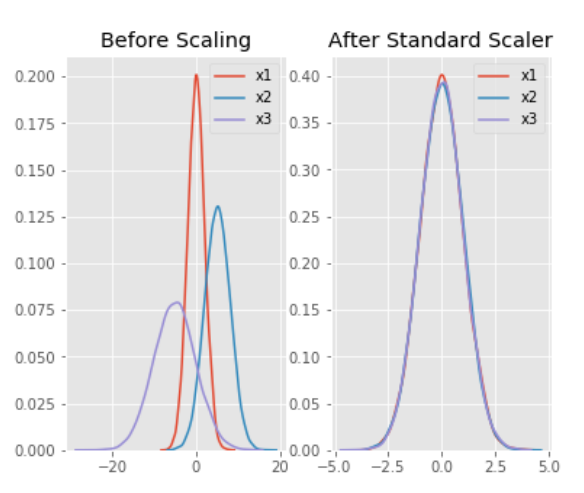
\includegraphics[width=0.4\textwidth]{standard-scaling.png}
    \caption{Voor en na standard scaling}
\end{figure}

\begin{figure}[H]
    \centering
    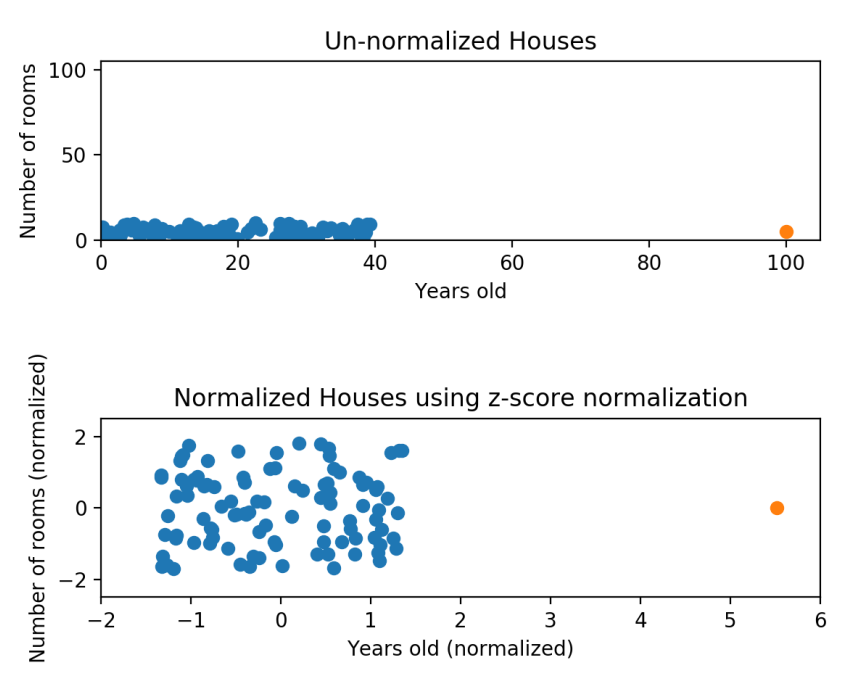
\includegraphics[width=0.4\textwidth]{standard-scaling-houses.png}
    \caption{Bij het voorbeeld van de huizenprijzen}
\end{figure}


\begin{minted}{python}
from sklean.preprocessing import StandardScaler

scaler = StandardScaler.fit(X_train)
X_train = scaler.transform(X_train)
X_test = scaler.transform(X_test)

# alternatief
scaler = StandardScaler()
X_train = scaler.fit_transform(X_train)
X_test = scaler.transform(X_test)
\end{minted}

\subsubsection{Robust scaling}

\begin{equation}
x_{s_i} = \frac{x_i - Q_2(x)}{Q_3(x) - Q_1(x)}
\end{equation}

\begin{itemize}
    \item Lijkt op MIN-MAX scaler maar gebruikt de interkwartielafstand ipv range
    \item Houdt geen rekening met uitschieters
    \item Gebruikt minder data bij het bepalen van de schaal
    \item Range van de genormaliseerde data is groter dan bij MIN-MAX scaling
    \item Garandeert geen genormaliseerde data op exact dezelfde schaal
\end{itemize}

\begin{figure}[H]
    \centering
    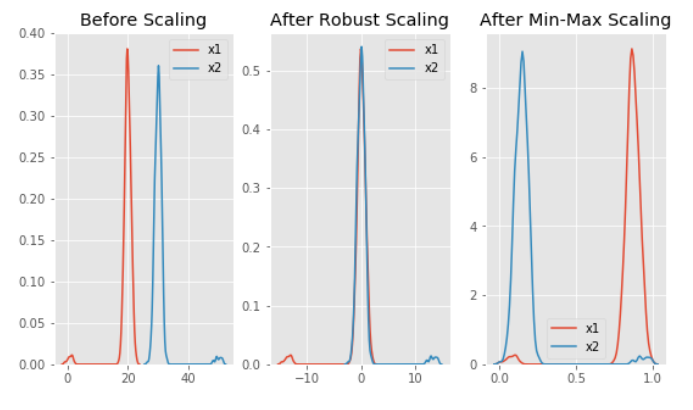
\includegraphics[width=0.45\textwidth]{robust-scaling.png}
    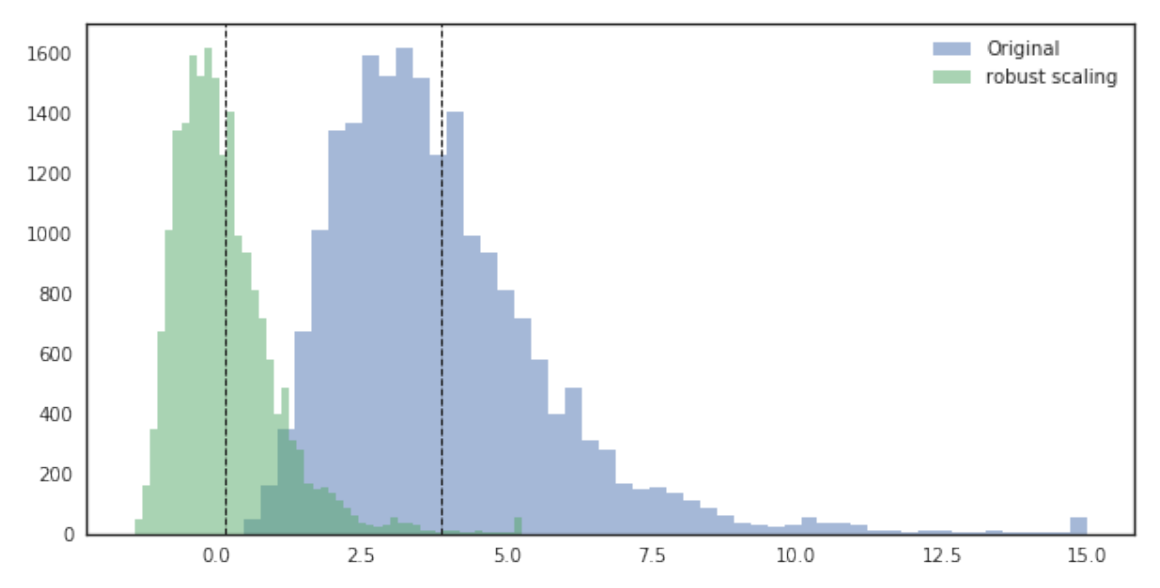
\includegraphics[width=0.45\textwidth]{robust-scaling2.png}
    \caption{Voor en na robust scaling}
\end{figure}

\begin{minted}{python}
from sklean.preprocessing import RobustScaler

scaler = RobustScaler.fit(X_train)
X_train = scaler.transform(X_train)
X_test = scaler.transform(X_test)

# alternatief
scaler = RobustScaler()
X_train = scaler.fit_transform(X_train)
X_test = scaler.transform(X_test)
\end{minted}

\subsection{Feature expansion}

\subsubsection{Nieuwe features}

Bedenken van nieuwe features

\textbf{Voorbeelden:}

\begin{itemize}
    \item Uit de lengte en breedte van een huis de oppervlakte halen als nieuwe feature.
    \item Uit een start en eindpunt de afstand halen als nieuwe feature.
    \item Uit een datum afleiden welke dag van de week het is.
    \item Veranderingen in de features.
    \item Nieuwe opgemeten parameters.
\end{itemize}

\subsubsection{Hogere-orde features}

= Het verband tussen features en de target(s) is niet altijd lineair.

\textbf{Voorbeeld:} samenhang tussen LSTAT $(x_1)$ en de huizenprijs $(P)$

\begin{figure}[H]
    \centering
    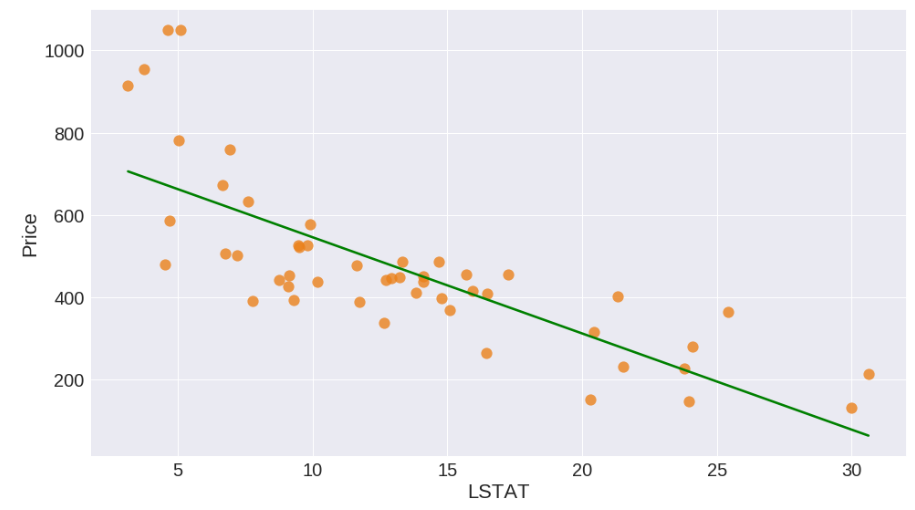
\includegraphics[width=0.3\textwidth]{hogere-orde-features.png}
    \caption{$P = \theta_0 + \theta_1x_1$}
\end{figure}

Toevoegen van een extra hogere-orde feature $x_2 = x^2_1$:

\begin{figure}[H]
    \centering
    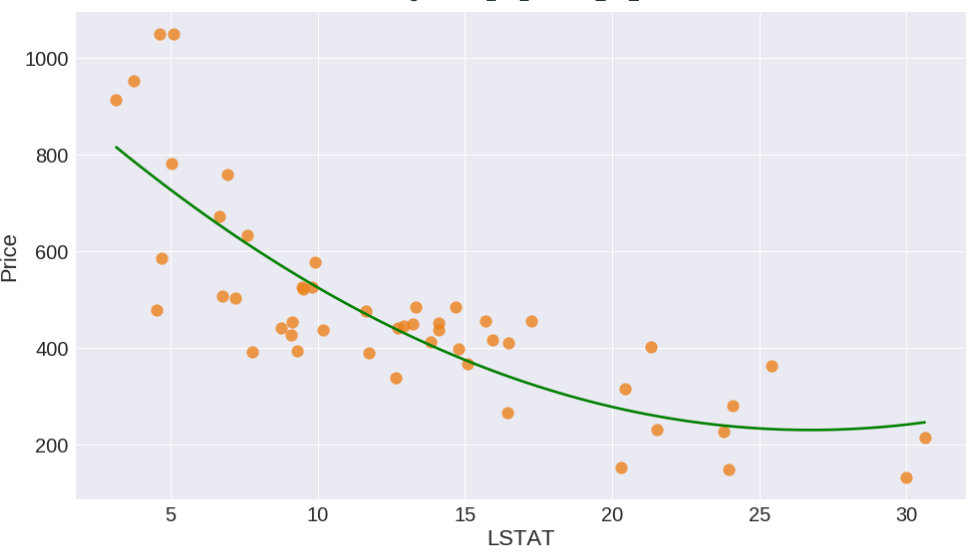
\includegraphics[width=0.3\textwidth]{hogere-orde-features2.png}
    \caption{$P = \theta_0 + \theta_1x_1 + \theta_2x_2$ }
\end{figure}

Toevoegen van een extra hogere-orde features $x_3 = x^3_1$ en $x_4 = x^4_1$:

\begin{figure}[H]
    \centering
    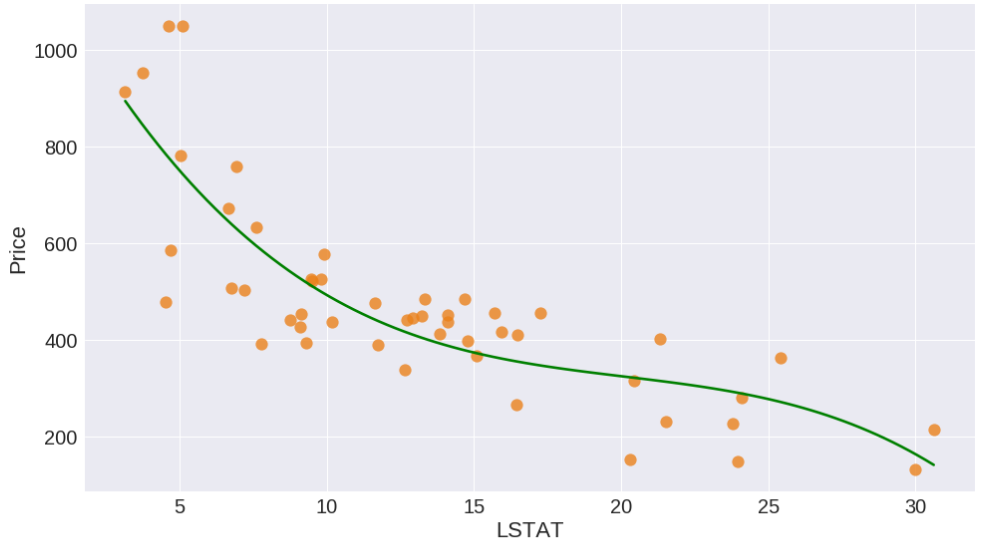
\includegraphics[width=0.3\textwidth]{hogere-orde-features3.png}
    \caption{$P = \theta_0 + \theta_1x_1 + \theta_2x_2 + \theta_3x_3$ }
    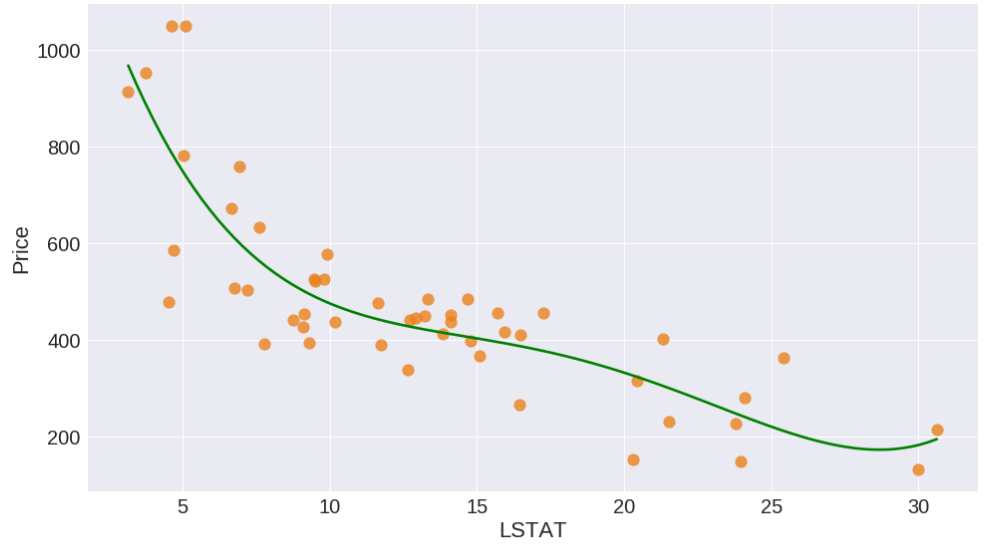
\includegraphics[width=0.3\textwidth]{hogere-orde-features4.png}
    \caption{$P = \theta_0 + \theta_1x_1 + \theta_2x_2 + \theta_3x_3 + \theta_4x_4$}
\end{figure}

\begin{figure}[H]
    \centering
\end{figure}

\begin{minted}{python}
# toevoegen van een extra feature: LSTAT^2 LSTAT^3
dataset.insert(dataset.columns.size - 1, 'LSTAT^2', dataset.LSTAT**2)
dataset.insert(dataset.columns.size - 1, 'LSTAT^3', dataset.LSTAT**3)
\end{minted}

\begin{figure}[H]
    \centering
    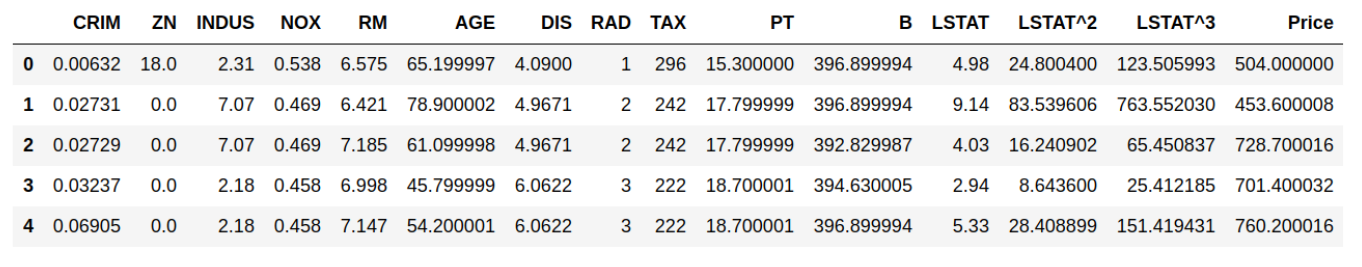
\includegraphics[width=0.5\textwidth]{hogere-orde-features5.png}
    \caption{Resultaat toevoegen hogere-orde features}
\end{figure}

\begin{itemize}
    \item Nu model met extra features trainen en nadien testen op de test set.
    \item \textbf{Opgepast:} bij de test set moet je ook dezelfde features toevoegen.
\end{itemize}

\subsection{One-hot encoding}

= Omzetten van categorische variabelen naar meerdere aparte features

(TODO: slide 94)



\end{document}